\documentclass[12pt]{book}

\usepackage{amssymb}
\usepackage{bbm}
\usepackage{dirtytalk}
\usepackage{hyperref}
\usepackage{subfig}
\usepackage{glossaries}
\usepackage{amsthm}
\usepackage{indentfirst}

\usepackage[style=authoryear, natbib=true]{biblatex}
\addbibresource{bibliography.bib}

\usepackage[section]{placeins}

\usepackage{tikz}
\usepackage{pgfplots}
\usetikzlibrary{positioning}
\tikzset{roundnode/.style={circle, draw=black!60, fill=white!5, very thick, minimum size=10mm},}

% Control TOC depth

\setcounter{tocdepth}{2}

% New Commands

\newcommand{\socrata}[2]{ 
\begin{tikzpicture}[node distance=3cm]
\node [roundnode] (#1) {#1};
\node [roundnode] (#2) [right of=#1] {#2};
\draw[ultra thick, <-] (#1) -- (#2);
\end{tikzpicture}
}

\begin{document}

\begin{center}
  \Large \textbf{An Analysis of Pairwise Preference} \\
  \vspace{0.1in}
  \normalsize Daniel Kronovet dbk2123\\
  \today
\end{center}
  
\begin{center}  
\begin{quotation}
\textit{
	... seek not the depths of your knowledge with staff or sounding line.
	For self is a sea boundless and measureless.
	Say not, \say{I have found the truth,} but rather, \say{I have found a truth.}
	}
\end{quotation}
- Kahlil Gibran, \textit{\say{Self Knowledge}} 
\end{center}

\section{Introduction}
This thesis will explore \textit{pairwise preference}, a concept with applications in political science, economics, social science, and machine learning (\cite{jordan}, \cite{arrow}).
A ``pairwise preference'' is simply a preference for one item over another, given two items.

We will argue that such a representation is capable of capturing human subjectivity accurately and precisely.
We will also show that this representation is highly general, and that problems posed in this framework are amenable to many kinds of analysis.

\bigskip

The choice to explore this particular representation was motivated by a particular reading of the history of science.
In the \textbf{theoretical context} section, we will review aspects of this history of science and attempt to discern some key themes.
This section will motivate our investigation of pairwise preferences and predict some desirable theoretical properties.

In the \textbf{mechanics} section, we will present the basic elements of preference graphs.
We will demonstrate methods of analysis, drawing on tools from probability and linear algebra.
We will show how a large class of preference resolution problems can be set up within this general framework.

In \textbf{applications}, we will develop various algorithms for analyzing these types of graphs, and discuss their strengths and limitations.

In \textbf{future directions}, we will identify additional avenues of exploration. There are particularly interesting possibilities involving blockchain-based virtual machine (BBVM) technologies like Ethereum.

\section{Theoretical Context}

This section will introduce some broad and fundamental ideas, ultimately rediscovering some key aspects of what is known as \textit{process philosophy}.

To begin, we will develop the problem's context, drawing on work from a variety of fields, including cognitive science, computer science, mathematics, philosophy, and political economy.
In addition, we will look at past and current events to attempt to bring the current historical moment into focus.

\bigskip

Our argument will proceed as follows:

\begin{itemize}
	\item First, we will attempt to view the problem of human social organization through the lens of resources and communication.
	\item Then, we will describe a fundamental link between representation and computability.
	\item We will then turn to the role of analysis in society, and discuss ways in which analysis can fail.
	\item Next, we will connect ideas from philosophy and cognitive science, emphasizing the relational property of subjective mental concepts.
	\item Finally, we will argue that pairwise preferences are well-suited to the task of analyzing subjective preference
\end{itemize}

\subsection{A Schematic View}

\begin{center}
\begin{quotation}
\textit{Man is not an ant, conveniently equipped with an inborn pattern of social instincts.
	On the contrary, he seems to be strongly endowed with a self-centered nature.
	If his relatively weak physique forces him to seek cooperation, his inner drives constantly threaten to disrupt his social working partnerships.}
\end{quotation}
	- Robert Heilbroner, \textit{The Worldly Philosophers}, p18
\end{center}

Let us consider the problem of nonviolent coordination at scale.
Let us view this is a problem of preference resolution, and preference resolution as a problem of information flow.

In small communities, such as groups of friends, information flows easily across the human medium of language, and these communities are generally seen as capable of peaceful, mutually-beneficial coordination.
They resolve preferences easily, with few resources, and the results are generally satisfactory \citep{deacon}.

As communities grow larger, the amount of information increases and preferences become more complex and difficult to resolve.
Further, language loses efficiency as meaning fluctuates across groups.
This increase in problem scale and decrease in language efficiency leads to a need for new structure (such as a government) to manage this process and coordinate the members \citep{hobbes}.
Supporting new structure requires additional resources, or alternatively a more efficient utilization of existing resources.
If the community cannot acquire new resources or technology, we can expect the community to fracture, or for the nature of the coordination to become more oppressive, at least for some members of the community \citep{eisenberg}.

The use of the term \say{non-violent} might (reasonably) seem to suggest that its absence implies violence; we choose to interpret it less dramatically as a loss of personal freedom.
Consider a bleak workplace, in which workers have relatively little control over their work \citep{lin}.
Consider a bronze-age empire, in which large public works projects were built by coercing large segments of the population into service \citep{heilbroner}.

\bigskip

This is the schematic relationship: scale and nonviolence are opposed, given a fixed level of resources and technology.
Additional resources or more efficient structure can allow nonviolent coordination at a larger scale.
\say{Structure} can refer to both objective social forms (such as democratic institutions), or the organization of mental concepts (such as the notion of \say{democracy}).

This last century has seen great advances both in terms of resources and technology.
The majority of the preference-resolution structures found in liberal democracies predate these developments.
It would seem reasonable therefore that there exist some number of viable preference-resolution frameworks waiting to be developed.
Experiments in developing these frameworks are ongoing.
Recent success includes the use of the liquid democracy framework pol.is in Taiwan \cite{barry} and various applications of the suite of tools developed by the Stanford Crowdsourced Democracy Team (\cite{lee:2015}, \cite{aitamurto:2016}).

It is just such a framework that we will attempt to develop.
Our first step will be to establish and explore the fundamental relationship between representation and computation, showing that choice of representation has meaningful consequences for speed and quality of analysis.

\subsection{Representation and Analysis}

\subsubsection{An Historical Example}

Our modern base-10 numbering system, commonly known as the \say{Arabic} numbering system, has roots in in both the Middle East and India.
Originally developed in India, this numbering system was brought to the Middle East by (among others) the 9th-century Persian mathematician Al-Khwarizmi, via his \textit{On the Calculation with Hindu Numerals}.
Fibonacci, a 13th-century Italian mathematician, became aware of this text and became an advocate for this numbering system, arguing for its adoption in place of Roman numerals in his \textit{Liber Abaci} (\cite{ore} \cite{ferguson}).

Prior to the adoption of Arabic numerals, mathematics was done using Roman numerals (\cite{heilbroner} \cite{gowers}).
Roman numerals, while adequate for counting and basic addition and subtraction, were unwieldy for more complex operations like multiplication and division; hence the widespread use of the abacus as a computational tool.
To practitioners of this era, such operations would likely have been seen as \say{advanced}; problems involving these operations would have been \say{difficult}.
The adoption of the Arabic system allowed for previously challenging computations to be performed quickly, easily, and accurately; leading to an overall acceleration in the pace of mathematical development.

In the parlance of machine learning, we could argue that the abacus represents an optimization within a local optimum; the adoption of the new numbering system represents an escape from that optimum.
In this historical anecdote, we see a demonstration of a fundamental relationship: that between \textbf{representation} and \textbf{analysis}.
Analytical methods are defined in relation to one or another representation; changes in representation imply a change in the set of available analytic operations.
In addition, observe that changes in representation have no impact on the underlying world; nothing about the world changed to make multiplication easier.
These types of paradigm shifts occur with infrequent regularity in the sciences, and are a feature of scientific progress \citep{kuhn}.

\subsubsection{Contemporary Examples}

More routinely, the notion of transforming from one representation to another appears often in the computer science and industrial engineering literature; in the former, pertaining to problems and the algorithms which solve them, and in the latter, to optimization.

In computer science, a problem is said to \textit{reduce} to another if it can be shown that an instance of the first can be transformed into an instance of the second, while preserving truth conditions.

In optimization, there exists significant literature concerning solving problems represented in specific constrained (convex) forms: problems defined in these ways can be solved by computer relatively quickly and precisely.
Much of the skill in this field is being able to identify how a problem represented in some (arbitrary) form can be transformed into an equivalent convex optimization problem.

An problem that may be difficult to analyze in one form may become easy to analyze if converted into a different but provably equivalent form.
The ability to discern these relationships among problems is a key skill for researchers in these fields.

\bigskip

As observed by British computer scientist Philip Wadler \cite{wadler}: 

\begin{quotation}
\textit{
	Powerful insights arise from linking two fields of study previously thought separate.
	Examples include Descartes's coordinates, which links geometry to algebra, Planck's Quantum Theory, which links particles to waves, and Shannon's Information Theory, which links thermodynamics to communication.
	}
\end{quotation}

For a more current example, we can look at recent development in machine learning.
Graphical models, a formalism for representing and analyzing complex joint probability distributions as graphs, allowed for the mixing of analytic techniques from both statistics and computer science.
Problems that are difficult to solve for a probability distributions are may be easy to solve for an equivalent graph, and vice versa \citep{wainwright}.

An important clarification is that for problems which can \textit{in principle} be solved in several representations, one representation may allow for \textit{faster} solutions.
This is important because problems requiring hours or months of computation to solve are essentially unsolvable for applications needing results in minutes or days.

An interesting (but speculative) example comes to us via studies of the Wason selection task, in which participants are asked to solve logical reasoning problems by flipping cards.
Experiments have shown that such problems are difficult when presented abstractly, but become significantly easier when presented in terms of common social reasoning tasks \citep{cosmides}, suggesting that the link between representation and analysis extends to cognition.

\bigskip

We can extend this notion of representation and analysis to more general domains.
Natural language is a representation; the written word can be read and interpeted, but not analyzed with the precision of mathematics.
Images, music, and so on are also representations; each representation permits some modes of analysis and eliminates others.

In machine learning and optimization, it is very common to represent data as points in high-dimensional space.
A car, possessing \textit{weight, acceleration, horsepower, mpg}, and \textit{year}, can be thought of as a point in the five-dimensional space positive orthant, denoted $\mathbb{R}^5_+$.
Such representations allow for analysis using all of the tools of geometry and linear algebra.
These tools are powerful; much research has been conducted on methods for \textit{embedding} non-numeric data types into these types of space, for example via collaborative filtering or word embedding (\cite{mikolov} \cite{koren}).

\subsection{Mutual Information and Utility}

Let us place the concepts of representation and analysis on formal footing.

\subsubsection{The Data Processing Inequality}

If you have three variables, $\{X, Y, Z\}$, existing in a Markov relationship such that $X$ affects $Y$, and $Y$ affects $Z$:

\[
X \rightarrow Y \rightarrow Z
\]

Then the \textit{mutual information} (intuitively, the amount one variable tells you about another) between $Z$ and $X$ can never be more than the mutual information between $Y$ and $X$:

\[
I(X; Y) \geq I(X; Z)
\]

This is known as the \textit{data processing inequality} \citep{cover}, because we can think of $X$ as some sort of \say{true} world, $Y$ as some data (measurements) taken of the world, and $Z = f(X)$ is the result of some analysis process $f$ we perform on those measurements.
The data processing inequality states that no amount of analysis can produce information about the world not already present in the data itself.

At first glance, this may seem problematic --- after all, what is the point of data analysis if we can't learn anything new?
To understand why this makes sense, we need to think of an analysis $f$ not as providing new \textit{information}, but rather as taking existing information and \textit{converting} it into a more applicable form.
Consider an average over $n$ measurements:

\[
f(X) = \frac{1}{n} \sum_{i=1}^n X_i
\]

The average contains less \textit{information} than the original data (for example, by discarding all information concerning variance), but is nonetheless a concise and useful summary of an important aspect of the data.

\bigskip

This result has several implications.
First, it allows us to frame the general problem of optimization and machine learning as an exploration of the space of possible data analyses.
To illustrate this, let us present the data processing inequality in the language of machine learning:

\[
Y \rightarrow X \rightarrow \hat{Y} \Rightarrow I(X; Y) \geq I(\hat{Y}; Y)
\]

Here, we have the standard notation of $Y$ representing the true, unobservable world; $X$ represents some data set of measurements taken from that world, and $\hat{Y} = f(X)$ representing the result of some analysis $f$, which may be, among other things, prediction, classification, or structural description of the data $X$.

Problems in optimization and machine learning are generally represented in a common form: we have some goal, represented via a real-valued \textit{objective} or \textit{loss} function.
This function calculates some key metric, like the likelihood of a prediction or the magnitude of an error.
With this function, we can then compare various candidate data analyses, and select the one which does the best (by minimizing or maximizing this metric).
Formally, if we think of $L$ as our objective function, and $f$ being an analysis, then we are looking for an optimal analysis $f^*$ such that:

\[
L(f^*(X)) \geq L(f(X))
\]

$\forall f \in \mathcal{F}$, with $\mathcal{F}$ representing \textit{the set of all possible analyses}.
When $L$ is some type of error metric, we are likely optimizing some (potentially convex) function.
When $L$ is a type of likelihood, we are likely performing some form of statistical parameter estimation.
The role of $L$ is important, in that it is often the derivatives of $L$ that allows us to explore $\mathcal{F}$.
Much research in these fields can be seen as concerning itself with 1) developing new methods for exploring $\mathcal{F}$, and 2) developing new functions $L$ to facilitate progress with (1).

\subsubsection{Measurement}

Ultimately, our goal is knowledge: information about the world.
Taking the temperature with a thermometer, tagging animals in wildlife preserves, and writing essays can all be seen as efforts to represent symbolically --- to measure --- some aspect of the world.
The first key idea is that measurement and representation are fundamentally linked: a measurement is only interpretable as a form of symbolic representation.
The second key idea, proven by the data processing inequality, is that advances in measurement expands the space of possible analyses; conversely, the power of analyses is upper-bounded by the power of measurement.

\bigskip

For an historical example, consider the history of oncology.
In attempting to study cancer, progress was made most rapidly for Leukemia, largely due to the ease with which cancer could be measured in the blood \citep{mukherjee}.

For a timely real-world example, consider the ubiquity of mobile phone cameras and the influence such cameras have had on police accountability.
Ostensibly, police have been abusing minority populations for decades, if not for centuries or even millennia.
Progress on this issue was slow, in large part due to difficulty in measuring the problem.

Soon after mobile phone cameras became commonplace, reporting (measurement) of police violence increased dramatically, giving rise to national protest and the well-organized and influential Black Lives Matter movement.
In this example, it is easy to see how the critical factor was not change in the underlying world, nor exclusively the development of better organizing techniques, but rather innovations in methods of measurement.

\bigskip

Formally, let us think of a representation $r \in \mathcal{R}$ as a process applied to the world $Y$, resulting in some objective measurement (data) $X \triangleq r(Y)$.
The world is always at least as complex as the measurement (consider the example of a map vs a territory: a perfect map would necessarily be the size of the entire territory).
Most measurements are therefore information-discarding; our goal is therefore to find the measurement which discards the least information.

\bigskip

Given two measurements $r_1, r_2 \in \mathcal{R}$, if $r_1$ captures more information, then:

\[
I(Y; r_1(Y)) > I(Y; r_2(Y)).
\]

If would prefer to think of all $r$ as random functions (to incorporate the notion of measurement error), then the relation becomes:

\[
I(Y; \mathbb{E}[r_1(Y)]) > I(Y; \mathbb{E}[r_2(Y)]).
\]

We cannot actually evaluate $I(Y; r(Y))$, as $Y$ is not available for analysis except through $r(Y)$; it is necessarily a unknowable object.
This does not, however, mean that $r$ is beyond study.
Rather, we will evaluate $r$ indirectly, by seeing how it impacts downstream analysis.

The key point is that it may always be possible to find a better $r^*$; \textit{the existence of such an $r^*$ cannot be disproven.}

\bigskip

Recalling the data processing inequality and our historical examples, we see how transforming between representations does not increase information; rather, it allows for new kinds of analysis of existing information.
We can think of the process of transformation as applying a function

\[
g: X \rightarrow X^\prime
\]

$g \in \mathcal{G}$, which maps representation $X$ to $X^\prime$.
If this function is \textit{injective} (or \say{one-to-one}), then both representations contain the same amount of information.
The conversion between graphs and matrices is an example of this type of transformation.

If the function is not injective, then information will be lost during the transformation.
This transformation may still be desirable (and often is) if the target representation allows for more valuable task-specific analysis.
The conversion of natural language into a bag of words is an example of this type of transformation.

Formally, we can say that

\[
I(Y; X) \geq I(Y; g(X))
\]

$\forall g \in \mathcal{G}$. With this result in hand, it may seems like transforming between symbolic representations is pointless.
However, it may be the case that a transformed representation permits analysis in away the original does not.

Analysis of text often falls in this category.
Many techniques for textual analysis rely on conversions of large blocks of text into many small entities: either single words (bags of words) or local word groups (n-grams).
These entities are then counted, and the statistical properties of these counts are analyzed.

These types of analyses have yielded valuable results: Markov models of language and topic models are just two examples \citep{blei}.
We can also think about recommendation systems, in which individuals and items are typically embedded into high-dimensional Cartesian space, as a type of representation transformation \citep{koren}.

The utility of these models is hard to capture in the language of mutual information, as it is always true that:

\[
I(Y; r(Y)) \geq I(Y; g(r(Y))) \geq I(Y; f(g(r(Y))))
\]

To represent the utility of task-specific analysis, we will posit a task-specific \textit{utility function} $U_t$, whose domain is any arbitrary analysis, and range is $\mathbb{R}$.
This utility function is left intentionally general and can incorporate many factors, such as computability.
The subscript $t$ reflects the notion that utility is interpreted as a function of time (or more concretely, computer instructions).

\bigskip

For a concrete example, let us consider the classic problem of sorting.
Consider an unsorted array $X$ of $n$ integers, which we would like to sort.
We will compare two algorithms: insertion sort, denoted $f_i$, and quicksort, denoted $f_q$.
As insertion sort runs in time $O(n^2)$ and quicksort runs in time $O(nlogn)$, we can say that:

\[
U_{O(nlogn)}(f_q(X)) = U_{O(n^2)}(f_i(X))
\]

Further, we can say that:

\[
U_{O(nlogn)}(f_q(X)) \geq U_{O(nlogn)}(f_i(X))
\]

This example illustrates another important point: although we introduce $f$ as a very general function, utility is evaluated only with respect to concrete implementations.
Observe that an analysis $f \in \mathcal{F}$ assumes a particular representation as input; we make our notation more concise by subscripting: $f_g \in \mathcal{F}_g$.

\bigskip

For a second concrete example, let us consider the basic problem of indexing.
We have a linked list $X$ of $n$ elements, and will need to repeatedly access arbitrary elements by position.
We have three functions: $g_{l \rightarrow a}$, which converts a linked list to a contiguous array, $f_l$, which indexes over a linked list, and $f_a$, which indexes over an array. $g_{l \rightarrow a}$ has complexity $O(n)$, $f_l$ has complexity $O(n)$, and $f_a$ has complexity $O(1)$.
We can see that, for a single access:

\[
U_{O(n+1)}(f_a(g_{l \rightarrow a}(X))) = U_{O(n+1)}(f_l(X))
\]

If we need to access elements $k$ times, however, we will find that (assuming that $g_{l \rightarrow a}(X)$ is evaluated only once):

\[
U_{O(n+k)}(f_a(g_{l \rightarrow a}(X))) = U_{O(nk)}(f_l(X))
\]

We see how the transformation of representation can yield benefits in terms of utility over time.
Complexity analysis is nothing new; the value of this notation is the easy extension to approximate algorithms, which converge arbitrarily close to the \say{true} answer over time.
This notation also allows us to compare different classes of algorithms.
In image recognition, for example, deep neural networks have been shown to outperform most other algorithms, in terms of classification accuracy
These algorithms, however, are relatively slow to train.
$U_t$ allows us to compare these algorithms in a new way: a neural network might have more utility over a long time horizon, but a simpler algorithm could have higher utility if time were limited.

\bigskip

The problem is therefore one of finding a transformation and analysis \textit{pipeline} $f_g^*$ such that, $\forall f_g \in \mathcal{F}_g$:

\[
U_t(f_g^*(X)) \geq U_t(f_g(X))
\]

In optimization, for example, problem constraints are often \say{relaxed} to allow for fast solutions which assume convexity.
We can think of these relaxations as information-discarding transformations which increase \textit{overall} utility by allowing for fast analysis.
Incorporating notation from earlier, we are ultimately interested in functions $r^*$ and $f_g^*$ such that:

\[
U(f_g^*(r^*(Y))) \geq U(f_g(r(Y)))
\]

$\forall r \in \mathcal{R}$,  $\forall f_g \in \mathcal{F}_g$. Ranging across all $g$ and $f$, we see that for each task-specific utility $U$, it may always be possible to develop some new $r^*$ such that:

\[
U(f_g(r^*(Y))) \geq U(f_g(r(Y))).
\]

In other words, in addition research in methods of analysis ($f$, $L$), we can conceive of research in methods of representation and measurement ($r$, $g$).
The development of new measurements has the potential to unlock more powerful types of downstream analysis, by capturing more information about the underlying world.
Note that we have \textit{not} shown that:

\[
I(Y; r^\prime(Y)) \geq I(Y; r(Y)) \rightarrow U_t(f_g^\prime(r^\prime(Y))) \geq U_t(f_g(r(Y)))
\]

for some $f_g^\prime, f_g \in \mathcal{F}_g$.
This is due to the varied interaction between representation and computability; there is no guarantee that an information-capturing representation will be easier to analyze; the opposite may be true.
However, a high information-capturing representation can always be converted into a simpler form; better measurements can only improve overall analytic ability.

\bigskip

In 1984, statisticians Persi Diaconis and David Freedman published a paper on the topic of \say{projection pursuit}.
In this paper, they show that an arbitrary projection of a high-dimensional random variable into a lower-dimensional space will with high probability exhibit a Gaussian distribution, regardless of the distribution of the original random variable \citep{diaconis}.
The Gaussian, or \say{normal}, distribution, is the maximum-entropy distribution for a random variable, given the variance of that variable.
Put another way, a variable that is normally distributed contains less information than one with any other continuous distribution.
Put yet another way, projection into lower dimensions very likely discards information.
Put a final way, \textit{the process of measurement itself can be seen as a process of projecting information from  some complex, unknown space (the true world) onto a finite-dimensional representational space}; necessarily, information is lost.

This is unfortunate.
The benefits of projection (which can be thought of as data compression) are great: data becomes smaller and easier to store, transmit, and analyze.
If the original data has special structure which can be exploited, compression can occur (using techniques such as Principal Components Analysis or gZip) with as little as zero information loss.
In other cases, as first shown by Johnson and Lindenstrauss, random data compression can occur with acceptable loss of information \citep{dasgupta}.

The takeaway is that compression is more effective when it can exploit any \textit{special structure} of the object in the original space.
In the context of this argument, we conclude that \textit{measurement is more effective when the representation captures accurately any special structure of the aspect of the world being measured}.

\bigskip

\fbox{\begin{minipage}{30em}
\textbf{Glossary}

$\mathcal{R}$: Set of all measurement processes $r: Y \rightarrow X$

$\mathcal{G}$: Set of all transformations $g: X \rightarrow X^\prime$

$\mathcal{F}$: Set of all analyses $f: X \rightarrow f(X)$
\end{minipage}}

\subsection{Economic History}

Our story of representation and analysis is found in economic history.

Middle-age economies were simple.
These economies, based largely on barter and regional currencies, required participants to possess special domain knowledge of the region and the items involved in the exchange; participants without this knowledge struggled to participate \citep{heilbroner}.
The innovation of money price transformed economies by allowing for a standard, numeric representation of value.

This standard, consistent representation created the foundation for further economic innovations.
In the domain of bookkeeping, numerical prices allowed for the development of double-entry bookkeeping, enable the development and maintenance of business ventures on a larger scale \citep{ferguson}.
In the domain of finance, numerical prices allowed for the development of mathematical models of risk, which themselves allowed for the development of systems of loans and credit.
The development of credit can be seen as enabling the coordination of economic activity across not only space, but time.
These innovations -- made possible also by improved communications technology -- greatly increased the sophistication of human economic affairs.

\bigskip

The interpretation of price as a low-dimensional representation of information has long been appreciated (although not phrased in those terms).
Via the mechanism of price, disparate independent entities are able to coordinate activities; a revolution in economics came about when this type price-based coordination was argued to contribute to communal progress.
In his classic \textit{Wealth of Nations} \citep{smith}, Adam Smith described the \say{invisible hand} which emerges from decentralized self-interested economic activity to guide overall economic development.

Recognizing the challenge of a centralized measuring and analyzing of economic information, Hayek and his conservative contemporaries defended price-based free markets against Communist alternatives on the grounds that price systems allowed information to flow rapidly throughout large and decentralized economies \citep{hayek}.
Central planners Hayek argued, would fail to aggregate enough information to make optimal planning decisions.

\bigskip

In idealized settings, market-based coordination can be shown to be optimal (with regards to some accepted optimality criteria, of course).
In his classic paper \say{The Problem of Social Cost}, Nobel prize-winning economist Ronald Coase demonstrated that, in the presence of perfect information and zero transaction costs, problem involving externalities (like pollution) can be solved optimally by market forces \citep{coase}.

In his paper, Coase argues that, with perfect information about the externalities and no transaction costs, entities will bargain amongst themselves and ultimately arrive at a Pareto-efficient equilibrium, independent of the initial allocation of property rights.
He goes on to argue that, given real-world conditions of limited information about externalities and non-zero transaction costs, such equilibriums cannot be expected to emerge solely from bargaining between entities.
Additional structures (such as governments and legal systems) will be necessary, and such structures are biased towards initial holders of property rights, meaning that initial allocations of property rights will influence final outcomes (as historical experience has shown to be the case).
 
In this example, we can also see an example of one of our schematic relationships: that between cost and technology.
A problem for Coase's theory is that externalities can be difficult, if not impossible to measure.
To accurately price and account for negative externalities like pollution, these externalities must be accurately measured.
Sufficiently precise measurement may be impossible; else prohibitively expensive.
Improvements in technology (for example, in air or water sampling) should allow for more accurate measurement of externalities as lower cost, which by our proposed theory will allow more effective peaceful large-scale coordination (via a market system).

\bigskip

The strengths of markets are often appreciated; as are their drawbacks.
Observers of England's industrial revolution were horrified by the living conditions of urban workers.
Although admittedly overlooking the bleakness of rural life, critics of industrialization pointed out how little of the human element seemed to be present in the economic calculus of industry \citep{heilbroner}.
Observing the aftermath of the United State's Great Depression, economist John Maynard Keynes realized that unaided free markets would not necessarily bring about long-term economic growth.
The instability of markets and their tendency towards crashes was observed by other economists \citep{minsky}.

Overall, we seem justified in concluding that the measure of price was a radical development, allowing for vastly improved communication and coordination.
However, the efficient metric fails to capture very important information, and is therefore by itself insufficient for coordinating human activity.

\subsection{The Proxy Gap}

Imagine we have a library, and we would like to know how many books the library contains.
We count the number of books (discrete objects, implicitly defined as units of paper, binding, etc), and return the sum.
Overall, a straightforward process.

Now, imagine we have visitors to this library.
These visitors read books, and we would like to know how much they liked the books they read.
We might ask them to rate each book on a scale of 1-5. For each book, we average these scores to return an aggregate score.

In the first example, there is little question about the legitimacy of the measurement: although there is still possibility for error (perhaps two adjacent books are the same color and the shelf is poorly lit, and they are mistaken for a single book), the result can generally be seen as legitimate and authoritative.
In the second case, however, there is room to question: how well do these measurements reflect the true subjectivity of the readers?
In the first case, we were concerned with objective quantities; in the latter, subjective experiences, which are generally accepted as being difficult to measure.

\bigskip

The notion of the relationship between the measurement and the construct being measured is known as \textbf{validity}, and is central to social science.
Several notions of validity have been proposed over the years, with the notion of ``construct validity'' having emerged as the central and overarching type of validity \citep{cronbach:1955}.
Construct validity can be thought of as the correctness of the conceptualization of the construct of interest (such as ``integrity'' or ``intelligence''), and the quality of the link between that construct and the measure in question.
Assessing construct validity is a jointly theoretical and empirical task, with researchers appealing to various statistical methods to show that the results of measures of a certain construct are consistent and correlated \citep{campbell:1959}.
In the context of this work, we can think of this necessary statistical tests as being an \textit{additional layer of computation} needed to ensure that the measure is truly information-capturing.
In the language of utility developed earlier, we can see this layer of computation as decreasing the utility of this analysis by increasing the amount of computation needed to return valuable results.

\bigskip

An instructive example comes to us via the \textit{Likert scale}. 
A type of survey, this scale consists of a number of \textit{Likert items}, each asking the participant to answer a question by checking boxes such as \say{Strongly Agree}, \say{Strongly Disagree} and so on.
Likert scales are popular for their ease of use, but are controversial due to their (perceived) ease of abuse.
Specifically, practitioners often treat this ordinal scale as an interval scale, and further assume an equivalence between answer given and the quality of the subjective experience.
These types of methodological errors can lead researchers to come to erroneous conclusions \citep{jamieson:2004}.
Here again, we see how this measure necessitates an additional layer of statistical validation (such as ensuring that the distribution of answers is normal or uniform) before interpretation. 

\bigskip

Given the difficulty of representing and analyzing subjective experience and personal qualities, a common practice is to rely on easily-measurable objective \textit{proxies}.
American mathematician Cathy O'Neil discusses this practice at length, reviewing the use of measurement proxies in domains as diverse as education, hiring, credit, and criminal justice \citep{oneil}.
One of her main conclusions is that poorly-designed proxies facilitate the perpetuation of existing race and class inequalities.
Many have begun reaching similar conclusions in the last few years; research into \say{algorithmic fairness} is new and ongoing (\cite{tramer}, \cite{friedler}).

Moving forward, we will refer to this gap between a measurement proxy and the stated object of measurement as the \textit{proxy gap}.
Returning to the library example, the book count has a proxy gap of (near) zero, as the measurement accurately captures the aspect of the world it purports to measure.
The book ratings, however, have a meaningful proxy gap: there are aspects of book preference which are not captured on a 1-5 scale.

Statistician David \citet{freedman} discusses an analogous concept:

\begin{quotation}
\textit{
	Regression models are widely used by social scientists to make causal inferences; such models are now almost a routine way of demonstrating counter-factuals.
	However, the \say{demonstrations} generally turn out to depend on a series of untested, even unarticulated, technical assumptions.
	Under the circumstances, reliance on model outputs may be quite unjustified.
	Making the ideas of validation somewhat more precise is a serious problem in the philosophy of science.
	That models should correspond to reality is, after all, a useful but not totally straightforward idea --- with some history to it.
	Developing models, and testing their connection to the phenomena, is a serious problem in statistics.
	}
\end{quotation}

By definition, the proxy gap is a qualitative, not quantitative, property.
As such, we will use it as a tool for developing the arguments to follow, but will abstain from attempting to incorporate it formally into analysis.
Still, the notion will be useful, as it provides a common frame with which to reason about potential failures of mathematical models of the world.

\subsubsection{Education}

As an example, let us consider some aspects of the American higher education system.

Prospective undergraduates are faced with a choice of several hundred possible universities -- too many to reasonably research and evaluate.
Clearly, there was a need for some sort of summary assessment of school quality. In 1983, in response to a perceived need, the \textit{US News \& World Report} released the first edition of their now-infamous college rankings \citep{oneil}.
Taking into account a number of factors, such as student test scores, acceptance and retention rates, and alumni giving, \textit{US News} generated a score, which it used to rank schools.
This ranking has, for better or worse, become a standard measure by which colleges are judged.

These rankings became so influential that schools began going to extreme (even illegal) lengths to improve their scores: lying about student test scores, building multi-million dollar athletic facilities (increasing tuition costs accordingly), and rejecting candidates deemed \say{unlikely to attend} \citep{oneil}.
Observe that these changes have unclear, if not outright negative, impact on \say{school quality}.

 In this example, the proxy gap is the gap between the actual measurements (student statistics) and the aspect of the world we are interested in (\say{school quality}).
 Because of this gap, incentives are distorted and it becomes possible to game the system.
 Schools are able to rise in the rankings without improving their quality, while other schools might fall in the rankings even as quality of education improve, if the improvements do not manifest in specific ways.

\bigskip

Standardized testing plays a huge role in controlling access to higher education.
These tests exist at all levels of education (SAT for undergraduates, GRE, LSAT, MCAT, GRE, and GMAT for graduate students).
These tests purport to measure academic aptitude for their respective courses of study; they are each a proxy with an associated proxy gap.

This proxy gap has lead to large test preparation industries.
In all cases, prospective students can be found eagerly signing up for test preparation courses, drilling practice questions and studying the standard structures of the test in question.
Students with access to resources (such as preparation courses) generally perform better; thus, critics say that these tests are at least in part measuring socioeconomic status \citep{zumbrin}.

\bigskip

In these examples, we see how the issue of \textit{legitimacy} of measurements becomes a major issue.
Measurements exhibiting large proxy gaps are easier to challenge as illegitimate.
This illegitimacy becomes a source of tension, as the illegitimacy of measurements calls into doubt the legitimacy of the systems built on those measurements.
As data and data processing becomes increasingly central to our activities, we should be attuned to the issue of legitimacy in modeling.

What insights can we draw from the examples given?
A general theme is a desire to measure subjective qualities.
In light of the earlier discussion on representation and measurement, it would seem we would benefit from some representation able to capture this subjective quality.
Representations of subjectivity exist already: language and art being two important examples.
In fact, language was the first symbolic representation, far predating any mathematical symbolism.

What these representations lack, however, is formality.
The formalisms of mathematics have allowed for the precise communication of fantastically complex ideas.
It should seem that we would like a representation combining the formality of math with the subjectivity of language.

\subsection{The Dialectic}

To develop our argument, we must first introduce some ideas of Hegel.
A german \say{idealist}, Hegel believed that concepts, and human conceptual structures, played a key role in determining the course taken by society.
Contrast these ideas with those of materialists, such as Marx, who believed that resource constraints ultimately shaped social forms.
Historical experience has, fortunately, shown that both views contains much truth; the experience of the Anabaptists in Munster following the Protestant Reformation \citep{carlin} shows clearly the power of ideas in shaping events, while the experience of the Israeli Kibbutzim points to the power of material conditions.

In developing his theory of ideas, Hegel articulated the concept of a dialectic.
In a dialectical process, we begin with an idea, known as the \textit{thesis}.
In contraposition to the thesis, there emerges an opposing idea, known as the \textit{antithesis}.
Thesis and antithesis engage in tension, the space between them one of paradox.
This tension is ultimately resolved into a new idea, the \textit{synthesis}.
This synthesis then plays the role of thesis to begin a new dialectical process.
Hegel contended that this process was helical, and thus contributed a forward momentum to human affairs.

We note that Hegel himself did not use the language of thesis-antithesis-synthesis, but rather spoke of abstract-negative-concrete.

An important aspect of a dialectic is that the thesis and antithesis are in opposition to each other, but neither is \say{correct} or \say{incorrect}.
We experience dialectics regularly in our lived experience:

\begin{enumerate}
  \item Freedom vs Security
  \item Individual vs Community
  \item Change vs Stability
  \item Process vs Outcome
\end{enumerate}

The recurrence of these themes in theater and literature attests to the fundamental role the dialectical structure plays in our shared and individual experiences.

Fundamentally, a dialectic is a paradoxical space between two contradictory extremes.
Resolving these tensions is an important part of our decision-making process.
As an example, we can view any political process (or smaller scale group decision-making processes) as being exercises in resolving these tensions into concrete actions.

Contrast a dialectic dimension with something like $\mathbb{R}$, the real line.
$\mathbb{R}$ is also a space in between two extremes: $-\infty$ and $\infty$.
The key difference is that \textit{numerical space is well-defined, while dialectical space is by definition contradictory.}

We argue that \textit{concepts are ultimately relational in nature, and that attempts to represent them in reference to some absolute scale inevitably obfuscates important aspects of their character.}

The Hegelian dialectic is not without critics.
Karl Popper, an eminent philosopher of science, has attacked dialectical thinkers for their willingness to accept, if not outright invite, contradictions \citep{popper}.
Popper, famous for his notion of \say{falsifiability} as a prerequisite property of valid scientific theories, felt that such conceptions of history were impossible to invalidate.

We resonate with Popper's emphasis on falsifiability.
Further, we agree with Popper's argument that contradictions are valuable primarily for their value in helping organizing our collective effort towards their resolution.
We believe a dialectical understanding is not in conflict with the scientific method, each being appropriate for making sense of one or another aspect of our experience.
Going further, we speculate that by continuously attempting to understand and resolve these paradoxes, dialectical distinctions can be made successively more nuanced.
We can imagine this as a \textit{recursive process}, by which distinctions are made nuanced, giving rise to further distinctions and further opportunities for nuance; this can be seen as the ideation process itself.

\bigskip

Returning to our earlier political example, it is easy to see dialectical tensions in the two-party system of the United States.
In the legislature, major dialectical themes such as \say{progress vs. stability} shape debate.
For the development of a specific policy, however, we should abhor contradiction; the budgets should balance.

\bigskip

The popular Myers-Briggs Type Indicator provides a useful case study of the power and pitfalls of the dialectical understanding.
This test asks a subject a series of questions, and then places them into one of two binary categories, along four axes.
Subjects are encouraged to see these categorizations as providing insight into their personality and their interactions with others.
This test appears often in popular culture and in business, and this popularity self-evidences the test's appeal.
Clearly, many find the test's structuring to be a valuable aid in their own thinking.

The test is not without critics.
Primary criticisms include low test-retest reliability, and of oversimplification and misunderstanding of complex personality traits.
These criticisms point to two important aspects of dialectical thinking:

\begin{enumerate}
	\item Any particular dialectic relationship represents a particular level of abstraction; any dialectical relationship can be made more nuanced. This relates to the dynamic, process-like nature of the dialectical relationship.
	\item Individuals experience reality differently. Descriptions of dialectic relationships are at best \textit{modal}, in that they describe common aspects of the experience of many, but not all.
\end{enumerate}

In seeking dialectical structure, the goal cannot be to learn a fixed and absolute structure. Rather, the goal must be to learn the particular task-specific structure (in terms of level of nuance) appropriate for the entities involved.

\subsection{Concept and Distinction}

Having introduced the sweeping notion of the dialectical process, how might we continue forward in developing a concrete theory?
It is too much to hope to be able to represent and formally analyze grand and abstract dialectical relationships.
What do we take with us?

First, we take the idea of \textit{distinction}, and take the notion of making distinctions between concepts as a fundamental operation.
Recalling momentarily our history of economics, we observe that it was not until the economic realm was \textit{distinguished} from the social and political realm could economic thinking take full flight \citep{heilbroner}.
Next, we accept the idea of a fundamentally process-like and relational nature of concepts; we should be cautious of approaches which attempt to embed these concepts in an absolute space.
Then, we ask whether these notions of distinction and relation can be applied to concepts more concrete than the grand abstractions often seen in introductions to dialectics.

\bigskip

Greek philosophers were preoccupied with understanding the true nature of things.
Heraclitus, a prominent pre-Socratic, believed that the true nature of things was \textit{change}: \say{you cannot step in the same river twice.}
Socrates and his students Plato and Aristotle felt differently: they felt that things were fundamentally constant and unchanging nature: \say{if Socrates gets sick, he is still Socrates.}

In his \say{Allegory of the Cave}, Plato defends this notion, arguing that the wide variation of things seen in the world is due to of physical objects being randomly-perturbed instantiations of constant, idealized types.
This Aristotelian orientation towards understanding phenomena in terms of fixed and constant properties has had significant influence on the development of science \citep{pirsig}.

\bigskip

Fast forward two millennia.
Leibniz dreamed of a language, \textit{characteristica universalis}, which could represent perfectly a wide variety of concepts in the world.
This language, \citet{couturat} writes, \say{would express the composition of concepts by the combination of signs representing their simple elements, such that the correspondence between composite ideas and their symbols would be natural and no longer conventional.}
Leibniz envisioned a future where disputes were settled by representing the problem as sentences in this universal language, and then simply \textit{calculating} the answer.
\say{Calculemus!}, he would say: let us calculate.

Many logicians who followed would attempt to develop similar systems for reasoning about discrete concepts and categories.
Ludwig Wittgenstein, however, recognized the impossibility of necessary and sufficient logical conditions for categories, and instead developed the idea of softer \say{family resemblances} among groups of things.

As an aside, we can see unsupervised approaches in machine learning (K-nearest neighbors, gaussian mixture models, and kernel-based approaches to classification being notable examples) as attempts to emphasize this relational quality.

\bigskip

An especially illustrative example comes to us in the form of Alfred North Whitehead.
A British mathematician and professor, Whitehead wrote the seminal \textit{Principia Mathematica} with his student, Bertrand Russell.
In \textit{Principia}, Whitehead and Russell sought to describe axioms and inference rules via which all mathematical truths could be proven \citep{doxiadis}.
A monumental endeavor, it was nonetheless a failure.
Kurt G{\"o}del, the German mathematician, showed that such systems were impossible: that any formal system contains unprovable truths \citep{hofstadter}.
Later in his career, Whitehead came to believe in the superiority of a \textit{process-based} ontology, in which objects in the world are understood not in terms of fixed, absolute characteristics, but rather as continuously undergoing change processes.
He would go on to write was has become the seminal text of process philosophy, \textit{Process and Reality} \citep{whitehead}.

\bigskip

These lines of thinking eventually transitioned from philosophy to cognitive linguistics, being pursued in the 1970s by the American linguist Eleanor Rosch, eventually culminating in the development of \textit{Prototype Theory} (\cite{rosch:1973}, \cite{rosch:1975}).

What Rosch found was that concepts tended to organize into hierarchies, with general \textit{prototypes} being more readily available for cognition than specific instances.
These prototypes in general describe the salient aspects of the object: the prototype \textit{tree} captures a great deal of information about both subordinate types \textit{pine} and \textit{elm}.
Superordinate types fail to contain enough information: \textit{plant} fails to capture enough salient properties.

A frequent characteristic of prototypes is a mono-syllabic name.
Consider \textit{car} and \textit{tree}, both succinct aural representations.
Flower, while being bi-syllabic, is descended from the monosyllabic Old French \textit{flor}.

\begin{figure}[hbt]
\begin{center}
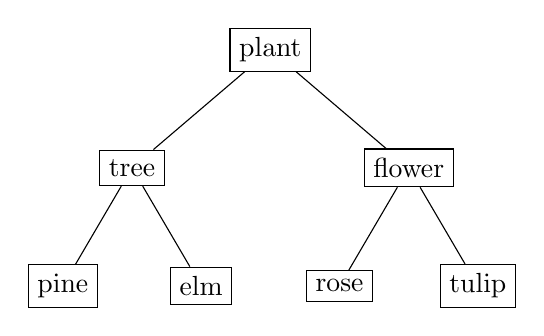
\begin{tikzpicture}[
  every node/.style = {shape=rectangle, draw, align=center},
   level 1/.style={sibling distance=10em},
   level 2/.style={sibling distance=5em}
    ]
  \node {plant}
    child { node {tree}
      child { node {pine} }
      child { node {elm} } }
    child { node {flower}
      child { node {rose} }
      child { node {tulip} } };
\end{tikzpicture}
\end{center}
\caption{Example conceptual tree}
\end{figure}


\begin{figure}[hbt]
\begin{center}
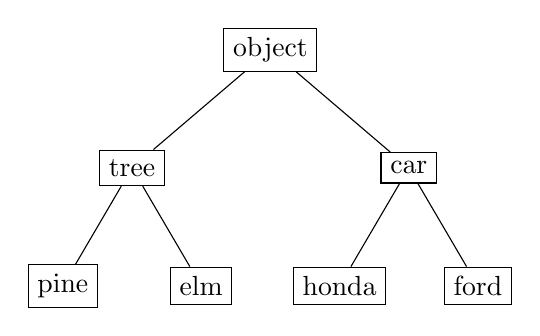
\begin{tikzpicture}[
  every node/.style = {shape=rectangle, draw, align=center},
   level 1/.style={sibling distance=10em},
   level 2/.style={sibling distance=5em}
    ]
  \node {object}
    child { node {tree}
      child { node {pine} }
      child { node {elm} } }
    child { node {car}
      child { node {honda} }
      child { node {ford} } };
\end{tikzpicture}
\end{center}
\caption{Alternative set of relationships}
\end{figure}

Rosch and others went on to show that culture and environment can effect what individuals come to understand as \say{prototypical}; in other words, how they come to distinguish experience.
For an individual raised in a forest, for example, the categories of \textit{pine} and \textit{elm} may in fact be prototypical categories.
For this individual, the differences between the two species are more salient than their similarities.
We can see this also in many professions: professionals communicate in jargon, making distinctions unfamiliar to those outside their field.

Rosch's work sheds a clarifying light on the relational nature of concepts.
What distinguishes \textit{tree} from \textit{elm} is not any particular property of \textit{elm}, but rather the presence of \textit{pine}.
If \textit{pine} did not exist, then \textit{elm} would add no information above and beyond that provided by \textit{tree}; \textit{elm} would not even exist.

American cognitive linguist \citet{lakoff03} develops Rosch's ideas in new directions, making central the idea of \textit{metaphor} in building understanding.
In Lakoff's view, complex ideas (distinctions) are understood by analogy from more basic ideas (distinctions).
A child, for instance, first comes to understand ideas of \textit{up} and \textit{down}, and \textit{warm} and \textit{cold}.
These first ideas are rooted in physical experience (the child has a body and experiences physical phenomena).
The child later comes to associate warmth with affection and cold with rejection (by observing the relationship between physical warmth and closeness to a parent, for example).

Once established, a child can come to understand more complex ideas by seeing them in terms of the more basic metaphors.
For example, imagine a child coming to understand a tumultuous friendship through the ideas of \say{hot} and \say{cold}.
For example, imagine a couple coming to understand their relationship as a journey they are on together.
The metaphoric nature of our understanding shapes politics, \citet{lakoff14} argues: candidates shape messages and choose words with care in their attempt to create advantageous associations in the minds of the electorate.

With these examples, we wish to show that the principles of distinction and opposition developed with regards to the dialectic can be applied more generally to mundane and everyday concepts.

\subsubsection{A Thought Experiment}

As a thought experiment, let's imagine a new intelligent agent, such as a human infant, or some hypothetical AI, has just come into existence.
Having been instantiated without assumptions, this agent possesses just one single, unified concept, extending infinitely in all directions.

The agent begins to experience a constant stream of stimulus, and must somehow learn how to navigate and act in the environment. What might this agent do? What operations are possible?

If the agent's entire understanding consists of a single concept, then the first thing the agent might do it \textbf{separate} that concept into two concepts.
The separation might be along some dimension, such that the two resulting concepts exist in some relation to each other.
Having successfully performed the separate operation, the agent could separate the resulting concepts again and again, recursively ad infinitum, each time along some new dimension, achieving an arbitrarily refined conceptual structure.

In understanding the \textbf{separate} operation, we have the notion of dimension.
Recalling Lakoff's basic metaphor, an early separation could be between left and right, or up and down -- basic distinctions needed to navigate physical environments.
As each separation is performed in sequence, we can also imagine a \textit{hierarchy} of separations, with earlier separations representing more fundamental distinctions, with later separations representing more fine-grained distinctions (within the framework established by earlier separations).

As a brief digression, it is thought-provoking to imagine this process of recursive conceptual definition as a sort of inverse of a traditional Buddhist or Hindu meditation practice.
In a meditation practice, one attempts to cease making distinctions in their experience. Here, we intentionally develop a system of distinctions recursively out of undifferentiated experience.


\subsection{Ordering and Pairwise Preference}

If we exhibit prejudice towards numerical representation, what alternatives might there be? Any candidate representation should satisfy the key criteria that \textit{the space between objects is left undefined.
}
Fortunately, item \textit{ordering} makes no statement about the nature of the relationship between the items, apart from their relative relations to each other.

\bigskip

Nobel prize-winning economist Kenneth Arrow has done extensive work analyzing voting systems.
Throughout much of his career, he advocated for ordinal representation of preference \citep{bianchi}, pointing out that relative preference is all that is naturally observed:

\begin{center}
	\begin{quotation}
\textit{
	The only evidence of an individual's utility function is supplied by his observable behavior, specifically the choices he makes in the course of maximizing the function.
	But such choices are defined by the preference order and must therefore be the same for all utility functions compatible with that ordering.
	\textbf{Hence there is no quantitative meaning of utility for an individual.}
	}
\end{quotation}
- Kenneth Arrow 1973; p104, emphasis added
\end{center}

However, Arrow would also show the limits of such a representation.
In his \textit{impossibility theorem}, Arrow proved that no ranked-choice system could satisfy all of a set of voting system criteria \citep{arrow}.
In light of this, Arrow would later amend his views and come to tolerate cardinal representations of preference, which contemplate real-valued distance between items, on the grounds that such representations provide additional information \citep{hamlin}.
Indeed, certain limitations of ordinal preference representation (such as the possibility of intransitive preference) are absent given cardinal preference representation.
However, Arrow cautioned against such systems, observing that wide ranges made it more likely that voters would misrepresent their preferences: \say{The trouble with methods where you have three or four classes, I think if people vote sincerely they may well be very satisfactory. The problem is the incentive to misrepresent your vote may be high.}

Interpreting Arrow's comments through our framework of representation and measurement, it seems as though we can interpret cardinal preferences as capable of representing more information.
We can see this is the case, given that we can always convert cardinal preferences to ordinal, but not vice versa.

This would seem to be a challenge for this thesis, which has been prejudiced against numerical representation of subjectivity.
If the question was only general expressiveness of representation, then the challenge would be severe.
Arrow's comments on error, however, point to a deeper tension: measurement error is almost certain to be higher for cardinal representations.

Returning to our formalisms, if we denote ordinal measurements with $r_o$, cardinal measurements with $r_c$, and the reduction of cardinal measurements to ordinal with $g_{c \rightarrow o}$, we see that:

\[
I(Y; r_c(Y)) \geq I(Y; g_{c \rightarrow o}(r_c(Y)))
\]

but 

\[
I(Y; r_c(Y)) \stackrel{?}{=} I(Y; r_o(Y))
\]

The latter uncertainty is due to the unknown trade off between expressiveness and measurement error.

\bigskip

We argue that pairwise preference has the advantage of being able to \textit{directly represent} subjectivity: a preference (or distinction) between two concepts.
This property emerges from the structured and limited nature of the pairwise preference: two items, and a preference for one over the other.
This representation does not by itself contain a huge amount of information, but what information is contained is an accurate reflection of the aspect of the world being represented: subjective preference.
We argue that, due to this direct representation, pairwise preferences are robust against measurement error; using terminology developed earlier, we can think of a pairwise preference as having a proxy gap of near-zero.
Regarding potential intransitivity of preference, seen as a major weakness for ordinal preference representation, we contend that such intransitivity is a feature of subjective experience, and we and seek to develop methods for recognizing and responding to intransitivity.
In the parlance of software engineering, \say{it's not a bug, its a feature}.

It is exactly for this ability of pairwise preference to directly represent subjectivity (and the contradictions that sometimes appear) that we choose to explore it.

\section{Mechanics}

\subsection{Elements}

Having concluded our survey of material and philosophical history, we are ready to develop the theory.
Our goal will be to develop a representation of subjective experience that is amenable to formal analysis.

Central to this theory will be the notion of pairwise preferences, which we have attempted to justify as a valid, yet formal, representation of subjective experience.

Before we can assess preference, we must establish some criterion to evaluate preferences against.
Among the same candidate set of answers, different questions can easily lead to different preferences.
For example, ranging over the items in your fridge, the questions \say{what to eat for breakfast} and \say{what to eat for dinner} will (likely) lead to different preferences among the same set of options.

\bigskip

We define questions with maximum generality, considering a general \say{question object} $Q$.
The representation of $Q$ is intentionally unspecified; the specific from of $Q$ will affect only the interpretation of the results, not the underlying theory.

We anticipate that $Q$ will often be represented via a string of characters (as in the fridge example).
However, $Q$ could be an image, a sound, an equation, or some new object yet unimagined.

\bigskip

In order to ask questions, we need candidate answers.
These candidate answers are members of an \textit{answer set} $A$.
As with the question object $Q$, the specific representation of the elements of $A$ are intentionally unspecified.

\bigskip

In order to represent subjective experience, we need an entity capable of subjective experience.
Discussions of subjectivity inevitably involve discussions of the notoriously elusive topic consciousness.
While the exact nature of consciousness is not known, researchers generally agree that conscious experience is attributed to discrete entities: as an entity I have an experience of consciousness that is separate from the experiences of other entities.
 
To resolve group preferences, we need a set of such discrete entities.
This set of entities is denoted $E$.
Unsurprisingly and in the spirit of this exposition, we leave the specific nature of these entities intentionally unspecified.
We anticipate that these entities will often be people. Later in this work we will introduce potential new directions for this theory, for which we may want to define these entities differently. Specifically, we will see how the problem of defining entities can be understood as selecting an \say{access policy}, the choice of which will shape the interpretation of the results.

\bigskip

Having introduced questions, answers, and entities, we are ready to introduce the \say{preference}, conceived of as a basic unit of subjective experience. As the name suggests, a preference represents an \textit{answer to a question}. Preferences have five components:

\begin{enumerate}
	\item A question object $Q$.
	\item An entity $e \in E$.
	\item A candidate answer $\alpha \in A$.
	\item A second candidate answer $\beta \in A$.
	\item The preference $p \in \{0, 1\}$, where $0$ corresponds to preferring $\alpha$.
\end{enumerate}

It is not immediately obvious how we might operate on this representation. Recalling that preferences are only defined relative to a question $Q$, we can make $Q$ implicit. Further, for the moment let us assume that we are interested only in the preferences of a single entity $e$.

Now, we see that the salient attributes of a preference are the two options $\alpha, \beta$, as well as the preference $p$. If we imagine $\alpha$ and $\beta$ as nodes, then $p$ can be represented as a directed edge between the two. Specifically, we create an edge $(\beta, \alpha)$ if $p = 0$ or $(\alpha, \beta)$ if $p = 1$ (the edge flows from loser to winner):

\begin{center}
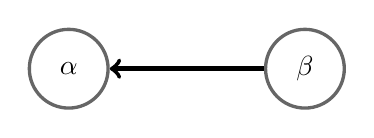
\begin{tikzpicture}[node distance=3cm]
\node [roundnode] (a) {$\alpha$};
\node [roundnode] (b) [right of=a] {$\beta$};
\draw[ultra thick, <-] (a) -- (b);
\end{tikzpicture}
\end{center}

This graphical representation is desirable, as it suggests a natural way of aggregating preference. Imagine we have $A = \{a, b, c, d\}$, and an entity $e$ generates the following preferences:

\begin{center}
\socrata{a}{b}
\socrata{a}{c}

\socrata{b}{d}
\socrata{c}{b}

\end{center}

We can aggregate these preferences into the following \textit{preference graph} $S$:

\begin{center}
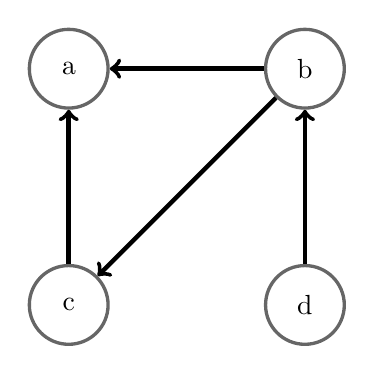
\begin{tikzpicture}[node distance=3cm]
\node [roundnode] (a) {a};
\node [roundnode] (b) [right of=a] {b};
\node [roundnode] (c) [below of=a] {c};
\node [roundnode] (d) [right of=c] {d};
\draw[ultra thick, ->] (b) -- (a);
\draw[ultra thick, ->] (c) -- (a);
\draw[ultra thick, ->] (d) -- (b);
\draw[ultra thick, ->] (b) -- (c);
\end{tikzpicture}
\end{center}

Aggregating preferences across multiple entities presents little difficulty.
If we have entity $\alpha$ generating the following (an ordered preference of $a, b, c$):

\begin{center}
\socrata{a}{b}
\socrata{a}{c}
\socrata{b}{c}
\end{center}

And entity $\beta$ generating the following (an ordered preference of $a, c, b$):

\begin{center}
\socrata{a}{b}
\socrata{a}{c}
\socrata{c}{b}
\end{center}


We can assign each preference a weight of 1 and combine the edges.
Parallel edges sum, while antiparallel edges cancel:

\begin{center}
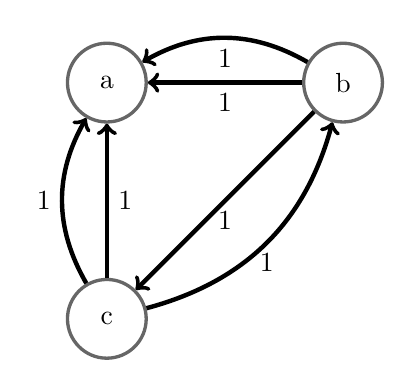
\begin{tikzpicture}[node distance=3cm]
\node [roundnode] (a) {a};
\node [roundnode] (b) [right of=a] {b};
\node [roundnode] (c) [below of=a] {c};
\draw[ultra thick, ->] (b) to[bend right] node[below] {1} (a);
\draw[ultra thick, ->] (b) -- node[below] {1} (a);
\draw[ultra thick, ->] (c) to[bend right]  node[below] {1} (b);
\draw[ultra thick, ->] (b) -- node[below] {1} (c);
\draw[ultra thick, ->] (c) to[bend left]  node[left] {1} (a);
\draw[ultra thick, ->] (c) -- node[right] {1} (a);
\end{tikzpicture}
\hspace{5mm}
\raisebox{2 cm}{$\rightarrow$}
\hspace{5mm}
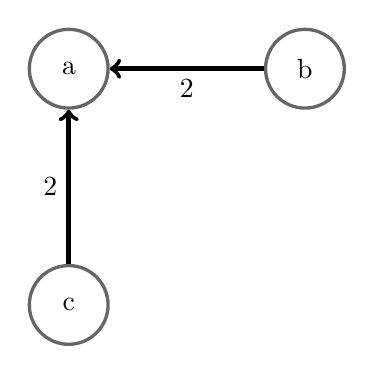
\begin{tikzpicture}[node distance=3cm]
\node [roundnode] (a) {a};
\node [roundnode] (b) [right of=a] {b};
\node [roundnode] (c) [below of=a] {c};
\draw[ultra thick, ->] (b) -- node[auto] {2} (a);
\draw[ultra thick, ->] (c) -- node[auto] {2} (a);
\end{tikzpicture}
\end{center}

It is instructive to see what occurs in the instance of two entities with opposing preferences.
Say we $\alpha$ with preferences $(a, b, c)$, and $\beta$ with preferences $(c, b, a)$.
We might say we could resolve this by selecting $b$, as this seems the mutually-agreeable option.

Is this principled?
Selecting $b$ would cause both entities to have their second preference, a forfeiting of one item each.
Selecting $a$ or $c$, on the other hand, would cause one entity to have its first preference, and the other third --- a forfeiture of two items.
In a sense, this pair of opposing preferences render all answers equal.

Observe what happens in the corresponding preference graph:

\begin{center}
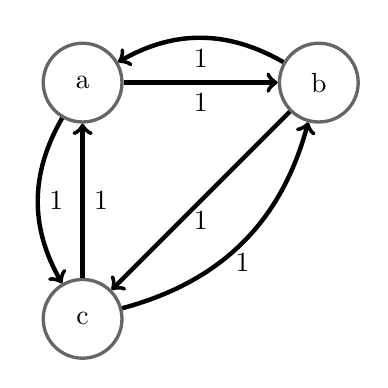
\begin{tikzpicture}[node distance=3cm]
\node [roundnode] (a) {a};
\node [roundnode] (b) [right of=a] {b};
\node [roundnode] (c) [below of=a] {c};
\draw[ultra thick, ->] (b) to[bend right] node[below] {1} (a);
\draw[ultra thick, ->] (a) -- node[below] {1} (b);
\draw[ultra thick, ->] (c) to[bend right]  node[below] {1} (b);
\draw[ultra thick, ->] (b) -- node[below] {1} (c);
\draw[ultra thick, ->] (a) to[bend right]  node[right] {1} (c);
\draw[ultra thick, ->] (c) -- node[right] {1} (a);
\end{tikzpicture}
\hspace{5mm}
\raisebox{2 cm}{$\rightarrow$}
\hspace{5mm}
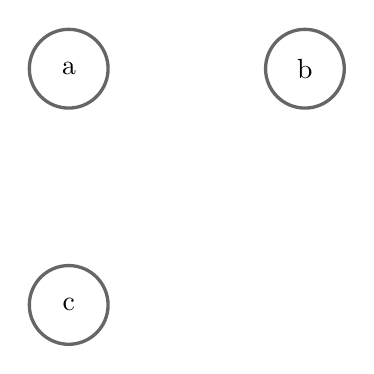
\begin{tikzpicture}[node distance=3cm]
\node [roundnode] (a) {a};
\node [roundnode] (b) [right of=a] {b};
\node [roundnode] (c) [below of=a] {c};
\end{tikzpicture}
\end{center}

The answers are disconnected; we interpret as an absence of preference.

\bigskip

\textit{A note on method:} we have been very intentional in our avoidance of assigning numerical value to subjective preference.
For an \textit{individual} entity (with an emphasis on the literal meaning of \say{individual} as non-divisible), preference is non-numeric.
Populations have magnitudes, however, and so we can comfortably reason in terms of sums and ratios when considering aggregations of entity preferences.

\subsection{A Probabilistic View}

Let us now consider some structural properties of preference graphs, and interpret them through the lens of preference resolution.
In this discussion, we will employ the elements of probabilistic methods of Paul \cite{erdos:1959}.

\bigskip

In the language of computer science, we denote graphs as $G = (V, E)$, with graph $G$ consisting of some set $V$ of \textit{vertices} (or \textit{nodes}) and some set $E$ of \textit{edges} between the vertices.
Edges can be directed or undirected, and are denoted $(u,v) \in E$, with $u, v \in V$.
When analyzing complexity, we use $n = |V|$, the number of vertices, and $m = |E|$, the number of edges.
We done the number of incoming edges for node $u$ as $in(u)$, and the number of outgoing edges as $out(u)$.
We refer to $in(u)$ as the ``indegree'' of $u$, and $out(u)$ as the ``outdegree'' of $u$.
Since an edge may exist between any pair of edges, we see that $m \leq n^2$.
In our case, there are ${n}\choose{2}$ possible pairs per graph.
Further, we see that $max_{u \in V}in(u) = n - 1$.

A vertex can be called a \textit{universal sink} if it has $in(u) = n - 1$.
In the context of preference, a universal sink is an option that is preferred over all others.
As a first pass, we can think of the problem of resolving preference as a problem of finding a universal sink, which can be found in O(n) time.

It might seem as the problem of preference resolution is simple: observe preferences, and find the universal sink.
Unfortunately, there is no guarantee that a universal sink will exist.

\bigskip

To show this, we will extend the $G(n,p)$ notation of Erd{\H o}s to the tournament graphs of \cite{landau:1953}.
A $G(n,p)$ graph is a random undirected graph of $n$ nodes, with the probability $p$ of an edge existing between any two nodes.
In this discussion, we will repurpose this notation to describe a different type of graph, a \textit{random tournament} $G_T(n,p)$, generated as follows:

\begin{enumerate}
	\item Create a complete graph of $n$ nodes.
	\item Remove all $(u,u)$ edges.
	\item Create a directed graph by randomly orienting the edges, with probability $p$ that $(u, v) \in E$ and probability $1-p$ that $(v, u) \in E$.
\end{enumerate}

We will show that as $n$ increases, the likelihood of a universal sink existing in a random tournament decreases exponentially.
Every vertex has $n-1$ edges.
For vertex $u$, to be a universal sink, all of these edges must point towards it.
If we consider a random tournament $G_T(n,p)$, then

\[
p(u_{usink}) = \prod_{v \in (V / \{u\})}p((u,v) \in E) = \frac{1}{2^{n-1}}
\]

Since the relationships between any pair of vertices is independent of all other pairs, the probability of \textit{any} sink is bounded by the sum of the probabilities of the individual vertices being sinks:

\[
p(G_{usink}) \leq \sum_{u \in V}p(u_{usink}) = \frac{n}{2^{n-1}}
\]

The likelihood of a universal sink existing in a random tournament decreases exponentially as $n$ increases.
If a tournament has no universal sink, then there must exist at least one \textit{cycle} in the tournament.
A cycle is a subset of vertices and edges such that there exists a \say{path} of edges such that any vertex in the cycle is reachable from any other.
Here is the simplest cycle between three vertices:

\begin{center}
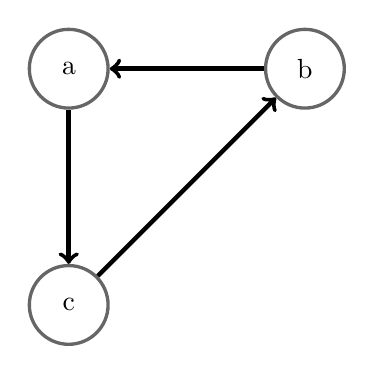
\begin{tikzpicture}[node distance=3cm]
\node [roundnode] (a) {a};
\node [roundnode] (b) [right of=a] {b};
\node [roundnode] (c) [below of=a] {c};
\draw[ultra thick, <-] (a) -- (b);
\draw[ultra thick, <-] (b) -- (c);
\draw[ultra thick, <-] (c) -- (a);
\end{tikzpicture}
\end{center}

It is easy to see that this tournament has no universal sink.
From the perspective of preference, we interpret a cycle as a set of items which are preferred equally; alternatively, we can say that they are \textit{indistinguishable} from each other.

If there are $n$ vertices, then there are $n\choose{2}$ pairs.
Since there are two possible states for each pair, there are a total of $2^{n\choose{2}}$ possible graphs.
As an illustration, let's consider a triple, where $n = 3$.For every triple of vertices, there are $2^3 = 8$ possible permutations of edges:

\begin{center}
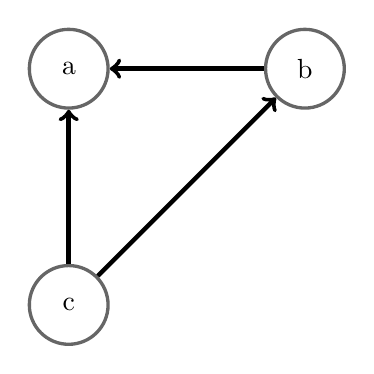
\begin{tikzpicture}[node distance=3cm]
\node [roundnode] (a) {a};
\node [roundnode] (b) [right of=a] {b};
\node [roundnode] (c) [below of=a] {c};
\draw[ultra thick, <-] (a) -- (b);
\draw[ultra thick, <-] (a) -- (c);
\draw[ultra thick, <-] (b) -- (c);
\end{tikzpicture}\quad
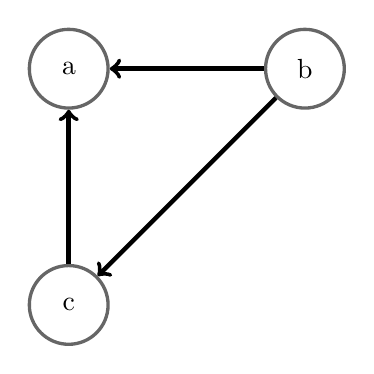
\begin{tikzpicture}[node distance=3cm]
\node [roundnode] (a) {a};
\node [roundnode] (b) [right of=a] {b};
\node [roundnode] (c) [below of=a] {c};
\draw[ultra thick, <-] (a) -- (b);
\draw[ultra thick, <-] (a) -- (c);
\draw[ultra thick, <-] (c) -- (b);
\end{tikzpicture} \quad
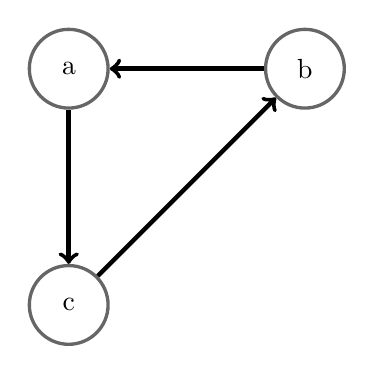
\begin{tikzpicture}[node distance=3cm]
\node [roundnode] (a) {a};
\node [roundnode] (b) [right of=a] {b};
\node [roundnode] (c) [below of=a] {c};
\draw[ultra thick, <-] (a) -- (b);
\draw[ultra thick, <-] (c) -- (a);
\draw[ultra thick, <-] (b) -- (c);
\end{tikzpicture}\vspace{5mm}
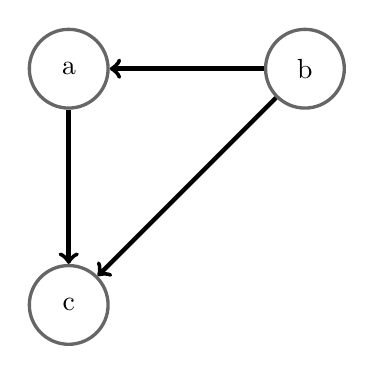
\begin{tikzpicture}[node distance=3cm]
\node [roundnode] (a) {a};
\node [roundnode] (b) [right of=a] {b};
\node [roundnode] (c) [below of=a] {c};
\draw[ultra thick, <-] (a) -- (b);
\draw[ultra thick, <-] (c) -- (a);
\draw[ultra thick, <-] (c) -- (b);
\end{tikzpicture} \quad
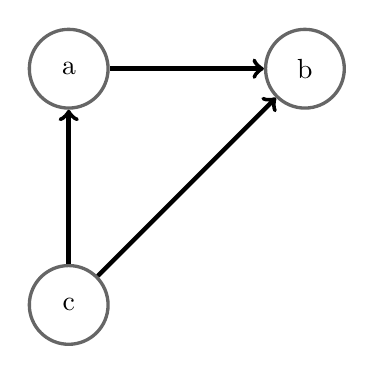
\begin{tikzpicture}[node distance=3cm]
\node [roundnode] (a) {a};
\node [roundnode] (b) [right of=a] {b};
\node [roundnode] (c) [below of=a] {c};
\draw[ultra thick, <-] (b) -- (a);
\draw[ultra thick, <-] (a) -- (c);
\draw[ultra thick, <-] (b) -- (c);
\end{tikzpicture}\quad
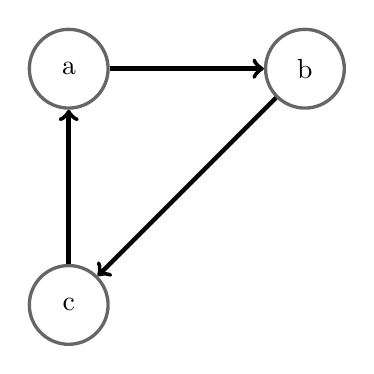
\begin{tikzpicture}[node distance=3cm]
\node [roundnode] (a) {a};
\node [roundnode] (b) [right of=a] {b};
\node [roundnode] (c) [below of=a] {c};
\draw[ultra thick, <-] (b) -- (a);
\draw[ultra thick, <-] (a) -- (c);
\draw[ultra thick, <-] (c) -- (b);
\end{tikzpicture} \vspace{5mm}
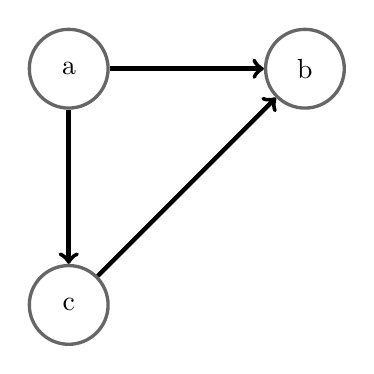
\begin{tikzpicture}[node distance=3cm]
\node [roundnode] (a) {a};
\node [roundnode] (b) [right of=a] {b};
\node [roundnode] (c) [below of=a] {c};
\draw[ultra thick, <-] (b) -- (a);
\draw[ultra thick, <-] (c) -- (a);
\draw[ultra thick, <-] (b) -- (c);
\end{tikzpicture}\quad
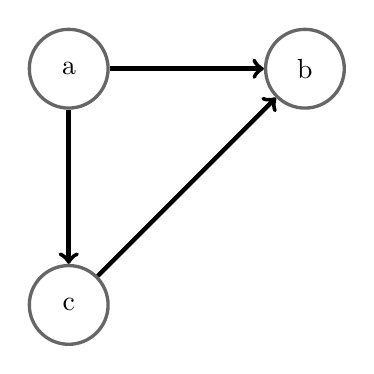
\begin{tikzpicture}[node distance=3cm]
\node [roundnode] (a) {a};
\node [roundnode] (b) [right of=a] {b};
\node [roundnode] (c) [below of=a] {c};
\draw[ultra thick, <-] (b) -- (a);
\draw[ultra thick, <-] (c) -- (a);
\draw[ultra thick, <-] (b) -- (c);
\end{tikzpicture}
\end{center}

In the case of three vertices, we see cycles in two out of eight possible graphs.
It is worth noting that while the absence of cycles in a random tournament necessarily implies the presence of a universal sink, the presence of a cycle does not necessarily imply the absence of a universal sink.
To see this, consider the following four-vertex directed graph:

\begin{center}
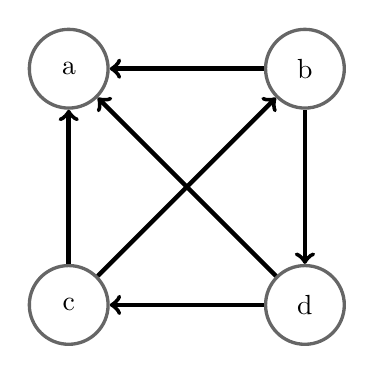
\begin{tikzpicture}[node distance=3cm]
\node [roundnode] (a) {a};
\node [roundnode] (b) [right of=a] {b};
\node [roundnode] (c) [below of=a] {c};
\node [roundnode] (d) [below of=b] {d};
\draw[ultra thick, <-] (a) -- (b);
\draw[ultra thick, <-] (a) -- (c);
\draw[ultra thick, <-] (a) -- (d);
\draw[ultra thick, <-] (b) -- (c);
\draw[ultra thick, <-] (c) -- (d);
\draw[ultra thick, <-] (d) -- (b);
\end{tikzpicture}
\end{center}

In this graph, vertices $\{c, b, d\}$ form a cycle, but $a$ is still a universal sink.
As discussed earlier, however, the likelihood of a universal sink existing in a random tournament, even allowing for cycles, decreases exponentially in $n$.

\bigskip

We raise this point to underscore that the presence of cycles does not imply the absence of meaningful structure; simply that meaningful structure will be more challenging to discern.
What is ``structure?''
American mathematician Claude Shannon defined a measure of structure, known as \textit{entropy}, which applied to probability distributions of random variables (\cite{cover}):

\[
H(X) = -\mathbb{E}[logp(X)] = -\sum_{x \in X}p(x)logp(x)
\]

Entropy is high when a distribution has a lot of uncertainty, and low when a distribution has little uncertainty.

This metric has proven invaluable: what analogous metrics might we develop for tournaments?
One possibility is the \textit{maximum indegree}, $max_{u \in V}in(u)$.
This metric can be calculated in $O(m + n)$ (linear time), and provides a rough sense of the amount of structure of the graph.

A second possibility is to look at the \textit{tournament entropy} $H_T$, the entropy of the empirical distribution of the indegrees of tournament $G$:

\[
H_T(G) = -\sum_{u \in V} \frac{in(u)}{m}log\bigg(\frac{in(u)}{m}\bigg)
\]

In the case of a three-node cycle, each node has an indegree of 1, equivalent to a uniform distribution over indegrees:

\begin{center}
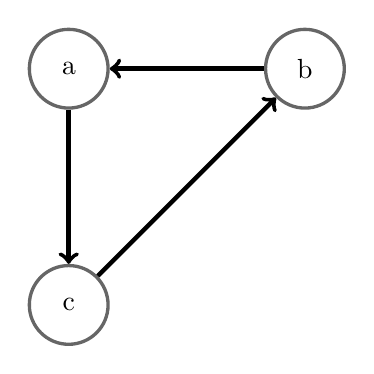
\begin{tikzpicture}[node distance=3cm]
\node [roundnode] (a) {a};
\node [roundnode] (b) [right of=a] {b};
\node [roundnode] (c) [below of=a] {c};
\draw[ultra thick, ->] (b) -- (a);
\draw[ultra thick, ->] (c) -- (b);
\draw[ultra thick, ->] (a) -- (c);
\end{tikzpicture}
\hspace{5mm}
\raisebox{2 cm}{$\rightarrow$}
\hspace{5mm}
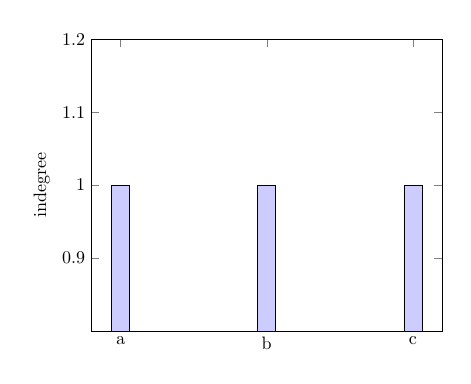
\begin{tikzpicture}[scale=0.65]
\begin{axis}[
    symbolic x coords={a, b, c},
    ylabel=indegree,
    xtick=data]
    \addplot[ybar,fill=white!80!blue] coordinates {
        (a,1)
        (b,1)
        (c,1)
    };
\end{axis}
\end{tikzpicture}
\end{center}

The tournament entropy of this graph is 1.585 bits, the maximum entropy distribution for three items.
In the case of a three-node transitive preference, we see a skewed distribution:

\begin{center}
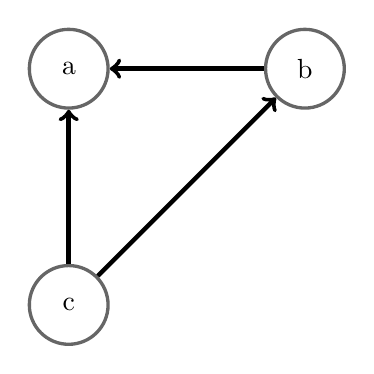
\begin{tikzpicture}[node distance=3cm]
\node [roundnode] (a) {a};
\node [roundnode] (b) [right of=a] {b};
\node [roundnode] (c) [below of=a] {c};
\draw[ultra thick, ->] (b) -- (a);
\draw[ultra thick, ->] (c) -- (b);
\draw[ultra thick, ->] (c) -- (a);
\end{tikzpicture}
\hspace{5mm}
\raisebox{2 cm}{$\rightarrow$}
\hspace{5mm}
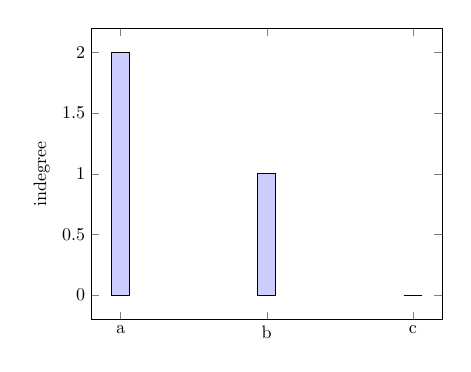
\begin{tikzpicture}[scale=0.65]
\begin{axis}[
    symbolic x coords={a, b, c},
    ylabel=indegree,
    xtick=data]
    \addplot[ybar,fill=white!80!blue] coordinates {
        (a,2)
        (b,1)
        (c,0)
    };
\end{axis}
\end{tikzpicture}
\end{center}

In this case, the tournament entropy is lower, only 0.918 bits.

\bigskip

We note that tournament entropy can be calculated in linear time.
Further, while this section has considered tournaments in which $m = {n\choose{2}}$ and every pair $\{u, v\}$ appears once, we can evaluate the tournament entropy of preference graphs with $m < {n\choose{2}}$ (graphs with partial observations), as well as thoughts with $m > {n\choose{2}}$ (graphs aggregating preferences of multiple entities).
When evaluating tournament entropy for preference graphs with large $m$, additional care must be taken as the distribution of observations across the pairs may not be uniform.

\subsection{A Linear Algebra View}

A graph can be represented as a matrix, with the values of the matrix corresponding to the values of the edges between nodes.
Let us denote the raw connection matrix as $C$.
By setting the values of the diagonal equal to the sum of their corresponding columns ($C_{ii} = \sum_j C_{ji}$), and normalizing the rows of this matrix ($\sum_i C_{ji} = 1$), we can construct a Markovian \say{transition matrix}, denoted $M$:

\begin{center}
\begin{minipage}{1.2in}
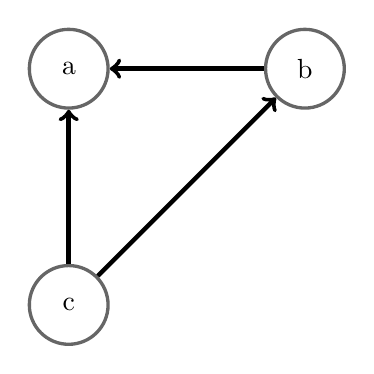
\begin{tikzpicture}[node distance=3cm]
\node [roundnode] (a) {a};
\node [roundnode] (b) [right of=a] {b};
\node [roundnode] (c) [below of=a] {c};
\draw[ultra thick, ->] (b) -- (a);
\draw[ultra thick, ->] (c) -- (b);
\draw[ultra thick, ->] (c) -- (a);
\end{tikzpicture}
\end{minipage}
\hfill
\begin{minipage}{1.2in}
\[
C=
  \begin{bmatrix}
    0 & 0 & 0 \\
    1 & 0 & 0 \\
    1 & 1 & 0
  \end{bmatrix}
\]
\end{minipage}
\hfill
\begin{minipage}{1.2in}
\[
M=
  \begin{bmatrix}
    1 & 0 & 0 \\
    .5 & .5 & 0 \\
    .5 & .5 & 0
  \end{bmatrix}
\]
\end{minipage}
\hfill
\end{center}



This matrix $M$ encodes the probability of ``transitioning'' from one item to another, with the values on the diagonal representing the likelihood of ``sticking with'' an item. 
If we imagine a vector $x_t \in \triangle^{V-1}$ representing the state at time $t$ as a distribution over all possible items, then

\[
x_{t+1} = x_t^TM
\]

gives us the distribution over items at time $t+1$.
If $M$ has certain properties (\textit{irreducible}, meaning that any item can be eventually reached from any other item, and \textit{aperiodic}, meaning that there are no stable loops among sets of states), then it can be shown that eventually $x$ will converge to a ``steady state'' distribution, in which $x = x^TM$ (\cite{lin:2016}).
Further, it can be shown that this steady state distribution, denoted $x_{\infty}$, is equivalent to the principal eigenvector of the matrix $M$, here denoted $v_1$.
The normalization of $M$ ensures that the principal eigenvector, denoted $\lambda_1$, is always equal to 1.

Interpreting $x_{\infty}$ as a distribution over items, then the components of $x_{\infty}$ with the largest values (probability) can be seen as the ``most preferred'' items.
The Perron-Frobenius theorem forms the foundation of these results, and use of this method has a long history (\cite{keener:1993}) and many applications, including the ranking of sports teams (\cite{landau:1915}) and websites (\cite{brin}).

\bigskip

It is worth discussing some interesting attributes of the principal eigenvector $v_1$.
First, by definition, $||v_1||_1$ (the $L_1$ norm) is equal to 1.
However, $||v_1||_2$ (the $L_2$ norm), varies.
Further, for $v_1$ with dimension $n$, $min(||v_1||_2^2) = n/n^2$, corresponding to a uniform preference over all items, and $max(||v_1||_2) = 1$, corresponding to a clear single preference.

\begin{proof}
As $||x||_2^2 \triangleq \sum x_i^2$, it will suffice to show that for any $\alpha \in \mathbb{R}, \epsilon > 0$,

\[
\bigg(\frac{1}{\alpha} + \epsilon\bigg)^2
+ \bigg(\frac{1}{\alpha} - \epsilon\bigg)^2
> \frac{2}{\alpha^2}.
\]

This is easily shown:

\[
\frac{1}{\alpha^2} + \frac{2\epsilon}{\alpha} + \epsilon^2
+ \frac{1}{\alpha^2} - \frac{2\epsilon}{\alpha} + \epsilon^2
 > \frac{2}{\alpha^2}
\]

\[
\frac{2}{\alpha^2} + 2\epsilon^2
 > \frac{2}{\alpha^2}
\]

\[
2\epsilon^2 > 0
\]
\end{proof}

This result suggests that $||v_1||_2$ can serve as an alternative measure of preference structure, with larger values implying more structured preference.
Further, for multiple entities, comparisons of entity-specific $v_1$ may be interpretable as comparisons of preference (entities with smaller distances between $v_1$ have more similar preferences, etc).
More work remains to be done understanding the specific behavior of $v_1$ and possible applications as a measure of preference structure beyond the standard application as a ranking.

\bigskip

With these concepts in hand, we can now ask what these steady states might look like for a series of simple preference graphs (Figures \ref{fig:linalg_1}, \ref{fig:linalg_2}, \ref{fig:linalg_3}, \ref{fig:linalg_4}, \ref{fig:linalg_5}, \ref{fig:linalg_6}).

% BEGIN LINALG FIGURES

\begin{figure}[!htb] % Two node transitive
\centering
\begin{minipage}{1.2in}
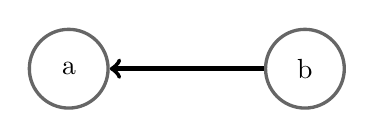
\begin{tikzpicture}[node distance=3cm]
\node [roundnode] (a) {a};
\node [roundnode] (b) [right of=a] {b};
\draw[ultra thick, ->] (b) -- (a);
\end{tikzpicture}
\end{minipage}
\hfill
\begin{minipage}{1.2in}
\[
M=
  \begin{bmatrix}
    1 & 0 \\
    1 & 0 \\
  \end{bmatrix}
\]
\end{minipage}
\hfill
\begin{minipage}{1.2in}
\begin{tikzpicture}
\def\v{2}
\def\x{2} % 2 * 1
\coordinate (O) at (0,0);
\coordinate (X) at (\x,0);
\draw [->] (O) -- (\v,0) node[below]{$x$};
\draw [->] (O) -- (0,\v) node[left]{$y$};
\draw [ultra thick, ->] (O) -- (X) node[right]{$v_1$};
\end{tikzpicture}
\end{minipage}
\caption{Preference graph $G$, transition matrix $M$, and principal eigenvector $v_1$ for a two-node transitive preference. $||v_1||_2^2 = 1$, $H_T(G) = 0$. Steady state achieved after one iteration.}
\label{fig:linalg_1} 
\end{figure}



\begin{figure}[!htb] % Two node cycle
\centering
\begin{minipage}{1.2in}
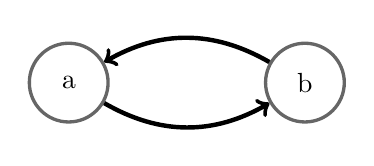
\begin{tikzpicture}[node distance=3cm]
\node [roundnode] (a) {a};
\node [roundnode] (b) [right of=a] {b};
\draw[ultra thick, ->] (b) to[bend right] (a);
\draw[ultra thick, ->] (a) to[bend right] (b);
\end{tikzpicture}
\end{minipage}
\hfill
\begin{minipage}{1.2in}
\[
M=
  \begin{bmatrix}
    .5 & .5 \\
    .5 & .5 \\
  \end{bmatrix}
\]
\end{minipage}
\hfill
\begin{minipage}{1.2in}
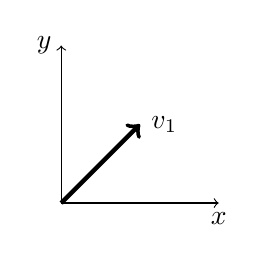
\begin{tikzpicture}
\def\v{2}
\def\x{1} % 2 * .5
\coordinate (O) at (0,0);
\coordinate (X) at (\x,\x);
\draw [->] (O) -- (\v,0) node[below]{$x$};
\draw [->] (O) -- (0,\v) node[left]{$y$};
\draw [ultra thick, ->] (O) -- (X) node[right]{$v_1$};
\end{tikzpicture}
\end{minipage}
\caption{Preference graph $G$, transition matrix $M$, and principal eigenvector $v_1$ for a two-node cycle. $||v_1||_2^2 = 1/2$, $H_T(G) = 1$. Intuitively, we set the probability of each item equal to the average of the prior preferences. The normalizing restriction on $v$ ensures that these averages continue to represent a distribution over the items. Note also that the steady state (a uniform distribution) is achieved after only one iteration.}
\label{fig:linalg_2} 
\end{figure}



\begin{figure}[!htb] % Three node transitive
\centering
\begin{minipage}{1.2in}
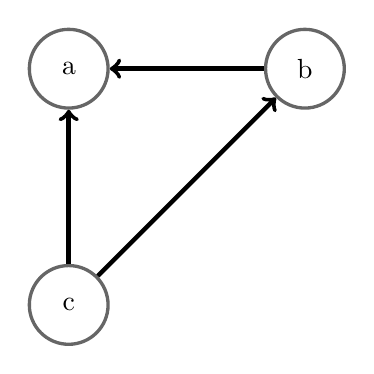
\begin{tikzpicture}[node distance=3cm]
\node [roundnode] (a) {a};
\node [roundnode] (b) [right of=a] {b};
\node [roundnode] (c) [below of=a] {c};
\draw[ultra thick, ->] (b) -- (a);
\draw[ultra thick, ->] (c) -- (b);
\draw[ultra thick, ->] (c) -- (a);
\end{tikzpicture}
\end{minipage}
\hfill
\begin{minipage}{1.2in}
\[
M=
  \begin{bmatrix}
    1 & 0 & 0 \\
    .5 & .5 & 0 \\
    .5 & .5 & 0
  \end{bmatrix}
\]
\end{minipage}
\hfill
\begin{minipage}{1.2in}
\begin{tikzpicture}
\def\v{2}
\def\x{2} % 2 * 1
\coordinate (O) at (0,0,0);
\coordinate (X) at (\x,0,0);
\draw [->] (O) -- (\v,0,0) node[below]{$x$};
\draw [->] (O) -- (0,\v,0) node[left]{$z$};
\draw [->] (O) -- (0,0,\v) node[below]{$y$};
\draw [ultra thick, ->] (O) -- (X) node[right]{$v_1$};
\end{tikzpicture}
\end{minipage}
\caption{Preference graph $G$, transition matrix $M$, and principal eigenvector $v_1$ for a three-node transitive preference. $||v_1||_2^2 = 1$, $H_T(G) = 0.918$. In this case, the steady state is achieved in the limit. At every iteration, C sends its probability mass to A and B evenly, and has no mass after the first iteration. B splits its mass between itself and A, while A directs all of its mass towards itself. The limiting convergence is due to the logarithmic reallocation of mass from B to A (a bit of a Zeno-style paradox).}
\label{fig:linalg_3} 
\end{figure}



\begin{figure}[!htb] % Three node cycle
\centering
\begin{minipage}{1.2in}
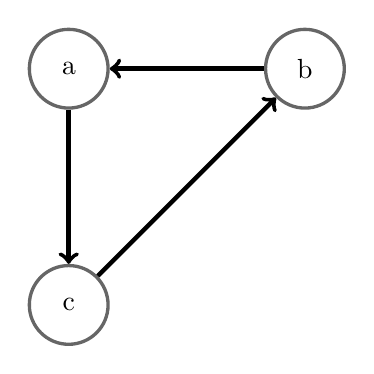
\begin{tikzpicture}[node distance=3cm]
\node [roundnode] (a) {a};
\node [roundnode] (b) [right of=a] {b};
\node [roundnode] (c) [below of=a] {c};
\draw[ultra thick, ->] (b) -- (a);
\draw[ultra thick, ->] (c) -- (b);
\draw[ultra thick, ->] (a) -- (c);
\end{tikzpicture}
\end{minipage}
\hfill
\begin{minipage}{1.2in}
\[
M=
  \begin{bmatrix}
    .5 & 0 & .5 \\
    .5 & .5 & 0 \\
    0 & .5 & .5
  \end{bmatrix}
\]
\end{minipage}
\hfill
\begin{minipage}{1.2in}
\begin{tikzpicture}
\def\v{2}
\def\x{.66} % 2 * 1/3
\coordinate (O) at (0,0,0);
\coordinate (X) at (\x,\x,\x);
\coordinate (Xxy) at (\x,0,\x);
\draw [->] (O) -- (\v,0,0) node[below]{$x$};
\draw [->] (O) -- (0,\v,0) node[left]{$z$};
\draw [->] (O) -- (0,0,\v) node[below]{$y$};
\draw [ultra thick, ->] (O) -- (X) node[right]{$v_1$};
\draw [dashed, color=red] (O) -- (Xxy);
\draw [dashed, color=red] (X) -- (Xxy);
\end{tikzpicture}
\end{minipage}
\caption{Preference graph $G$, transition matrix $M$, and principal eigenvector $v_1$ for a three-node cycle. $||v_1||_2^2 = 1/3$, $H_T(G) = 1.585$. Here the reallocation of probability mass across iterations exhibits more complex dynamics, and converges to $v_1$ in the limit.}
\label{fig:linalg_4} 
\end{figure}



\begin{figure}[!htb] % Three node double cycle
\centering
\begin{minipage}{1.2in}
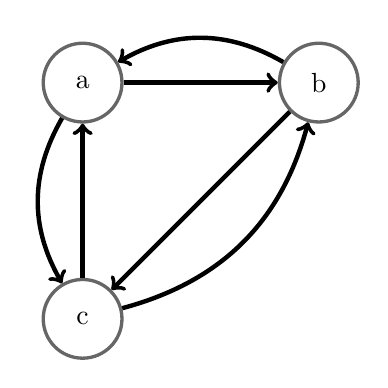
\begin{tikzpicture}[node distance=3cm]
\node [roundnode] (a) {a};
\node [roundnode] (b) [right of=a] {b};
\node [roundnode] (c) [below of=a] {c};
\draw[ultra thick, ->] (b) to[bend right] (a);
\draw[ultra thick, ->] (c) to[bend right] (b);
\draw[ultra thick, ->] (a) to[bend right] (c);
\draw[ultra thick, ->] (a) -- (b);
\draw[ultra thick, ->] (b) -- (c);
\draw[ultra thick, ->] (c) -- (a);
\end{tikzpicture}
\end{minipage}
\hfill
\begin{minipage}{1.2in}
\[
M=
  \begin{bmatrix}
    .5 & .25 & .25 \\
    .25 & .5 & .25 \\
    .25 & .25 & .5
  \end{bmatrix}
\]
\end{minipage}
\hfill
\begin{minipage}{1.2in}
\begin{tikzpicture}
\def\v{2}
\def\x{.66} % 2 * 1/3
\coordinate (O) at (0,0,0);
\coordinate (X) at (\x,\x,\x);
\coordinate (Xxy) at (\x,0,\x);
\draw [->] (O) -- (\v,0,0) node[below]{$x$};
\draw [->] (O) -- (0,\v,0) node[left]{$z$};
\draw [->] (O) -- (0,0,\v) node[below]{$y$};
\draw [ultra thick, ->] (O) -- (X) node[right]{$v_1$};
\draw [dashed, color=red] (O) -- (Xxy);
\draw [dashed, color=red] (X) -- (Xxy);
\end{tikzpicture}
\end{minipage}
\caption{Preference graph $G$, transition matrix $M$, and principal eigenvector $v_1$ for a three-node double cycle. $||v_1||_2^2 = 1/3$, $H_T(G) = 1.585$}
\label{fig:linalg_5} 
\end{figure}



\begin{figure}[!htb] % Three node transitive with edge weights
\centering
\begin{minipage}{1.2in}
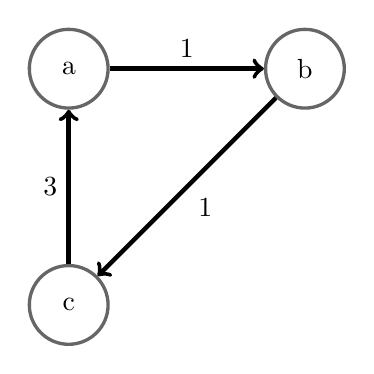
\begin{tikzpicture}[node distance=3cm]
\node [roundnode] (a) {a};
\node [roundnode] (b) [right of=a] {b};
\node [roundnode] (c) [below of=a] {c};
\draw[ultra thick, ->] (a) -- node[auto] {1} (b);
\draw[ultra thick, ->] (b) -- node[auto] {1} (c);
\draw[ultra thick, ->] (c) -- node[auto] {3} (a);
\end{tikzpicture}
\end{minipage}
\hfill
\begin{minipage}{1.2in}
\[
M=
  \begin{bmatrix}
    .75 & .25 & 0 \\
    0 & .5 & .5 \\
    .75 & 0 & .25
  \end{bmatrix}
\]
\end{minipage}
\hfill
\begin{minipage}{1.2in}
\begin{tikzpicture}
\def\v{2}
\def\a{1.09068489}
\def\b{0.54557228}
\def\c{0.36374283}
\coordinate (O) at (0,0,0);
\coordinate (X) at (\a,\c,\b);
\coordinate (Xxy) at (\a,0,\b);
\draw [->] (O) -- (\v,0,0) node[below]{$x$};
\draw [->] (O) -- (0,\v,0) node[left]{$z$};
\draw [->] (O) -- (0,0,\v) node[below]{$y$};
\draw [ultra thick, ->] (O) -- (X) node[right]{$v_1$};
\draw [dashed, color=red] (O) -- (Xxy);
\draw [dashed, color=red] (X) -- (Xxy);
\end{tikzpicture}
\end{minipage}
\caption{Preference graph $G$, transition matrix $M$, and principal eigenvector $v_1$ for a three-node cycle with edge weights. $||v_1||_2^2 = 0.4049$, $H_T(G) = 1.371$. Note how the introduction of variable weights repositions $v_1$ within the simplex, allowing us to recover a transitive ordering $a > b > c$.}
\label{fig:linalg_6} 
\end{figure}


\begin{figure}[!htb] % Four node two cycle
\centering
\begin{minipage}{1.2in}
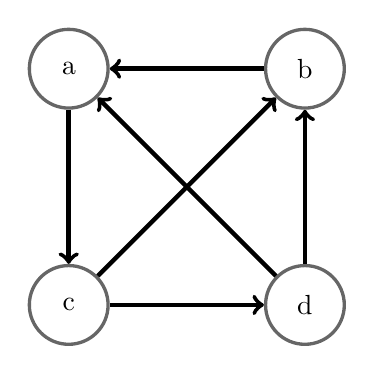
\begin{tikzpicture}[node distance=3cm]
\node [roundnode] (a) {a};
\node [roundnode] (b) [right of=a] {b};
\node [roundnode] (c) [below of=a] {c};
\node [roundnode] (d) [below of=b] {d};
\draw[ultra thick, ->] (a) -- (c);
\draw[ultra thick, ->] (b) -- (a);
\draw[ultra thick, ->] (c) -- (b);
\draw[ultra thick, ->] (d) -- (a);
\draw[ultra thick, ->] (d) -- (b);
\draw[ultra thick, ->] (c) -- (d);
\end{tikzpicture}
\end{minipage}
\hfill
\begin{minipage}{1.2in}
\[
M=
  \begin{bmatrix}
    .66 & 0 & .33 & 0 \\
    .33 & .66 & 0 & 0 \\
    0 & .33 & .33 & .33 \\
    .33 & .33 & 0 & .33
  \end{bmatrix}
\]
\end{minipage}
\hfill
\begin{minipage}{1.2in}
\[
(.4, .3, .2, .1)
\]
\end{minipage}
\caption{Preference graph $G$, transition matrix $M$, and principal eigenvector $v_1$ for a four-node graph with two cycles. $||v_1||_2^2 = 0.3$, $H_T(G) = 1.918$.}
\label{fig:linalg_7} 
\end{figure}


\begin{figure}[!htb] % Four node upper cycle
\centering
\begin{minipage}{1.2in}
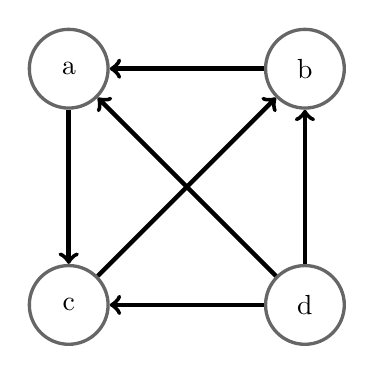
\begin{tikzpicture}[node distance=3cm]
\node [roundnode] (a) {a};
\node [roundnode] (b) [right of=a] {b};
\node [roundnode] (c) [below of=a] {c};
\node [roundnode] (d) [below of=b] {d};
\draw[ultra thick, ->] (a) -- (c);
\draw[ultra thick, ->] (c) -- (b);
\draw[ultra thick, ->] (b) -- (a);
\draw[ultra thick, ->] (d) -- (a);
\draw[ultra thick, ->] (d) -- (b);
\draw[ultra thick, ->] (d) -- (c);
\end{tikzpicture}
\end{minipage}
\hfill
\begin{minipage}{1.2in}
\[
M=
  \begin{bmatrix}
    .66 & 0 & .33 & 0 \\
    .33 & .66 & 0 & 0 \\
    0 & .33 & .66 & 0 \\
    .33 & .33 & .33 & 0
  \end{bmatrix}
\]
\end{minipage}
\hfill
\begin{minipage}{1.2in}
\[
(.33, .33, .33, 0)
\]
\end{minipage}
\caption{Preference graph $G$, transition matrix $M$, and principal eigenvector $v_1$ for a four-node graph with one cycle. $||v_1||_2^2 = 1/3$, $H_T(G) = 1.585$. Note that we see a cycle in $v_1$, despite having a larger $L_2$ value than the previous example.}
\label{fig:linalg_8} 
\end{figure}


\begin{figure}[!htb] % Four node lower cycle
\centering
\begin{minipage}{1.2in}
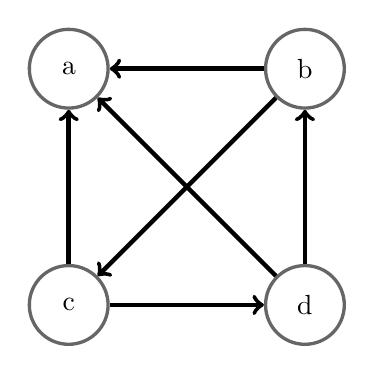
\begin{tikzpicture}[node distance=3cm]
\node [roundnode] (a) {a};
\node [roundnode] (b) [right of=a] {b};
\node [roundnode] (c) [below of=a] {c};
\node [roundnode] (d) [below of=b] {d};
\draw[ultra thick, ->] (b) -- (a);
\draw[ultra thick, ->] (c) -- (a);
\draw[ultra thick, ->] (d) -- (a);
\draw[ultra thick, ->] (b) -- (c);
\draw[ultra thick, ->] (c) -- (d);
\draw[ultra thick, ->] (d) -- (b);
\end{tikzpicture}
\end{minipage}
\hfill
\begin{minipage}{1.2in}
\[
M=
  \begin{bmatrix}
    1 & 0 & 0 & 0 \\
    .33 & .33 & .33 & 0 \\
    .33 & 0 & .33 & .33 \\
    .33 & .33 & 0 & .33
  \end{bmatrix}
\]
\end{minipage}
\hfill
\begin{minipage}{1.2in}
\[
(1, 0, 0, 0)
\]
\end{minipage}
\caption{Preference graph $G$, transition matrix $M$, and principal eigenvector $v_1$ for a four-node graph with one cycle. $||v_1||_2^2 = 1$, $H_T(G) = 1.793$. Note how the presence of a cycle in the lower nodes does not prevent the graph from having high level of structure.}
\label{fig:linalg_9} 
\end{figure}

% END LINALG FIGURES

This series of basic examples illustrate how the language of graphs and matrices allows us to make meaningful statements about preference in the presence of challenging structures like cycles, which manifest as contradictions when represented in terms of linear ordering.

\FloatBarrier

\subsection{Connections to Social Choice Theory}

Those readers familiar with the economics literature will see many parallels to the Social Choice Theory presented in \cite{arrow}.
In this work, Arrow proposed three criteria for good voting systems, and went on to famously prove that no voting system could exist which satisfied all three.
These criteria are:

\begin{itemize}
	\item \textbf{Unanimity}: if all voters prefer a to b, the group prefers a to b.
	\item \textbf{Non-dictatorship}: there is no individual voter whose preferences always prevail.
	\item \textbf{Independent of Irrelevant Alternatives (IIA)}: the group preference between a and b should be determined only by individual preferences between a and b (and not, for example, c).
\end{itemize}

Arrows impossibility theorem shows that these three criteria taken together can lead to contradiction.
We will give a sketch of the proof here (inspired by \cite{geanakoplos:2005}), as well as reinterpret the contradiction through the framework of preference graphs.

\bigskip

First, imagine we have a set $V$ of $N$ voters, asked to each submit a linear ordering of three items: $a, b$, and $c$.
The voters are partitioned into three sets as follows: $S_1 = \{V_1, ..., V_{k-1}\}$, $K = \{V_k\}$, and $S_2 = \{v_{k+1}, ..., V_N\}$, and all voters in each set always vote the same way.
Set $K$ consists of one voter, $V_k$, who we will refer to as the ``pivotal voter'' in that if $V_k$ votes the same way as either $S_1$ or $S_2$, then that preference prevails for the group.
In Figure \ref{fig:impossiblity_tables}, we see a sequence of three states of preference.
A contradiction emerges in the third state, when the preference reversals of $S_1$ and $S_2$ have no impact on the group preference.

\begin{figure}[!htb]
\centering
\begin{tabular}{ c | c | c | c }
 $S_1$ & $K$ & $S_2$ & Group \\ 
 \hline
 b & a & a & a \\ 
 c & b & b & b \\  
 a & c & c & c
\end{tabular}
 $\rightarrow$
\begin{tabular}{ c | c | c | c }
 $S_1$ & $K$ & $S_2$ & Group \\ 
 \hline
 b & \textbf{b} & a & \textbf{b} \\ 
 c & \textbf{a} & b & \textbf{a} \\  
 a & c & c & c
\end{tabular}
 $\rightarrow$
\begin{tabular}{ c | c | c | c }
 $S_1$ & $K$ & $S_2$ & Group \\ 
 \hline
 \textbf{c} & b & a & b \\ 
 \textbf{b} & a & \textbf{c} & a \\  
 a & c & \textbf{b} & c
\end{tabular}
\caption{Sequence of preference orderings for voter subsets $S_1$, $K$, and $S_2$, and final group preference. $V_k$ is a dictator in that the group prefers $b > c$ even though both $S_1$ and $S_2$ prefer $c > b$.}
\label{fig:impossiblity_tables} 
\end{figure}

In Figure \ref{fig:impossiblity_graphs}, we see the same sequence of preferences represented graphically.
In this view, we see that the ``paradox'' is simply the inability to represent cyclical preference as a linear ordering.
We also see how the IIA assumption becomes problematic, as the ordering of $b > a$ and $a > c$ inhibits the group ordering of $c > b$.
If we relax the IIA assumption and allow cycles, we see that the final preference graph of this proof has the same structure as our example graph in Figure \ref{fig:linalg_6}, and therefore has a steady state distribution of $c > a > b$.
Note that the eigenvector-based methods described earlier imply IIA relaxation.

\begin{figure}[!htb]
\centering
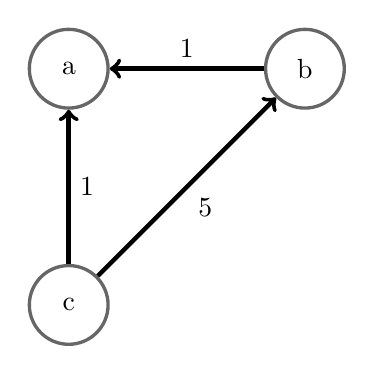
\begin{tikzpicture}[node distance=3cm]
\node [roundnode] (a) {a};
\node [roundnode] (b) [right of=a] {b};
\node [roundnode] (c) [below of=a] {c};
\draw[ultra thick, <-] (a) -- node[auto] {1} (b);
\draw[ultra thick, <-] (a) -- node[auto] {1} (c);
\draw[ultra thick, <-] (b) -- node[auto] {5} (c);
\end{tikzpicture}\quad
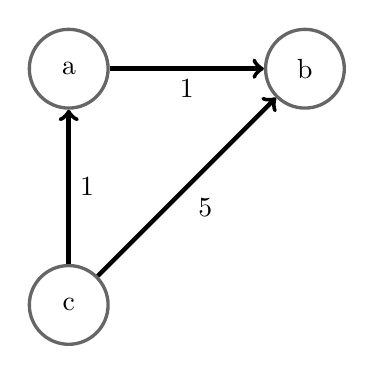
\begin{tikzpicture}[node distance=3cm]
\node [roundnode] (a) {a};
\node [roundnode] (b) [right of=a] {b};
\node [roundnode] (c) [below of=a] {c};
\draw[ultra thick, <-] (b) -- node[auto] {1} (a);
\draw[ultra thick, <-] (a) -- node[auto] {1} (c);
\draw[ultra thick, <-] (b) -- node[auto] {5} (c);
\end{tikzpicture} \quad
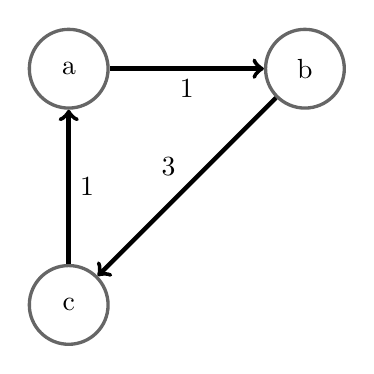
\begin{tikzpicture}[node distance=3cm]
\node [roundnode] (a) {a};
\node [roundnode] (b) [right of=a] {b};
\node [roundnode] (c) [below of=a] {c};
\draw[ultra thick, <-] (b) -- node[auto] {1} (a);
\draw[ultra thick, <-] (a) -- node[auto] {1} (c);
\draw[ultra thick, <-] (c) -- node[auto] {3} (b);
\end{tikzpicture}
\caption{Same sequence of preference orderings, shown as preference graphs. We set $|S_1| = |S_2| = 2$. $S_1$ and $S_2$'s reversal of preference between $b$ and $c$ in the third graph creates a cycle.}
\label{fig:impossiblity_graphs} 
\end{figure}

Here we see how the language of preference graphs clarifies the dynamics involved in social choice.


\section{Applications}

Ultimately, our goal is to make statements about the \textit{global} relationships which exist in the graph, using information which comes to us via \textit{local} relationships between nodes.
Arrow's IIA criteria requires the consideration of local relationships only, but as we have seen, this criteria is problematic in the presence of cyclic preference structure.

The graphical approach taken here relaxes this criterion and considers all items and preferences collectively.
However, accounting for global relationships between nodes (relationships involving three or more nodes) is computationally challenging due to the rapid increase in the number of subsets to consider.
For example, a graph of ten items has 45 pairs, 120 triples, and 210 sets of four.
Fully accounting for all possible interactions among items is currently computationally prohibitive for large graphs; as a result, techniques for approximately learning preference structure, or for pruning or otherwise constraining the number of items, will become valuable.

\subsection{Linear-Time Methods}

If a graph is not fully connected (some vertices lack edges), then it is possible for there to exist multiple sinks.
If a graph is fully connected, however, then there can exist at most one sink.
\footnote{\textbf{Proof}: if there are two sinks, one must point towards the other: contradiction $\rightarrow\leftarrow$.}

The first example we will consider is the most fundamental of preference resolution systems: the \textbf{plurality voting system}.
In this system, entities (which we will call voters) are allowed to vote for one of $n$ candidates, and the candidate with the most votes win.

To set up this system in the language of preference graphs, we will define the following:
Our \textit{access policy} is that every voter is allowed to cast one vote in the election.
Each vote will be translated into $n-1$ preferences, with an edge pointing to the chosen candidate from every other candidate.
For example, given three candidates $\{a, b, c\}$, a vote for $a$ would translate into the following:

\begin{center}
	
\socrata{a}{b}

\socrata{a}{c}
	
\end{center}

We aggregate the preferences using the additive rule described above.
The winner of the election will be the sink of the resulting graph.
The absence of cycles is guaranteed by the structure of the access policy.
Consider the following result: $a$ receives 10 votes, $b$ receives 7, and $c$ receives 3.
We combine these into the following graph:

\begin{center}
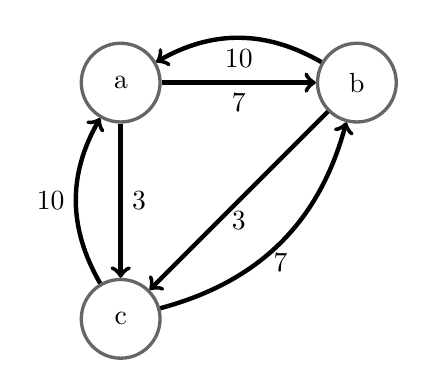
\begin{tikzpicture}[node distance=3cm]
\node [roundnode] (a) {a};
\node [roundnode] (b) [right of=a] {b};
\node [roundnode] (c) [below of=a] {c};
\draw[ultra thick, ->] (b) to[bend right] node[below] {10} (a);
\draw[ultra thick, ->] (a) -- node[below] {7} (b);
\draw[ultra thick, ->] (c) to[bend right]  node[below] {7} (b);
\draw[ultra thick, ->] (b) -- node[below] {3} (c);
\draw[ultra thick, ->] (c) to[bend left]  node[left] {10} (a);
\draw[ultra thick, ->] (a) -- node[right] {3} (c);
\end{tikzpicture}
\hspace{5mm}
\raisebox{2 cm}{$\rightarrow$}
\hspace{5mm}
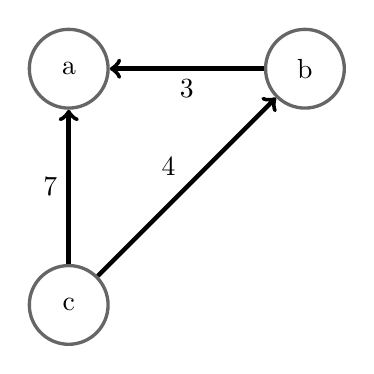
\begin{tikzpicture}[node distance=3cm]
\node [roundnode] (a) {a};
\node [roundnode] (b) [right of=a] {b};
\node [roundnode] (c) [below of=a] {c};
\draw[ultra thick, ->] (b) -- node[auto] {3} (a);
\draw[ultra thick, ->] (c) -- node[auto] {7} (a);
\draw[ultra thick, ->] (c) -- node[auto] {4} (b);
\end{tikzpicture}
\end{center}

We run the sink-finding algorithm and return $a$, the winner.
It is worth nothing how the complexity of this preference-resolution scheme is $O(n)$, the same as the complexity of simply taking the maximum of vote counts for $n$ candidates.

What happens in the case of a tie?
Let's say $b$ receives 10 votes:

\begin{center}
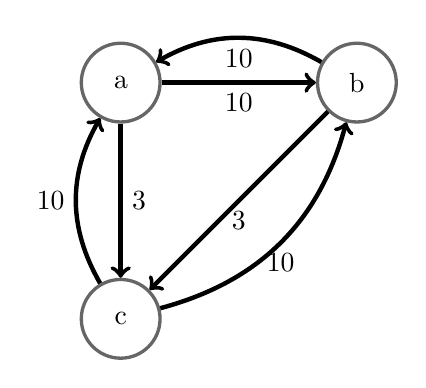
\begin{tikzpicture}[node distance=3cm]
\node [roundnode] (a) {a};
\node [roundnode] (b) [right of=a] {b};
\node [roundnode] (c) [below of=a] {c};
\draw[ultra thick, ->] (b) to[bend right] node[below] {10} (a);
\draw[ultra thick, ->] (a) -- node[below] {10} (b);
\draw[ultra thick, ->] (c) to[bend right]  node[below] {10} (b);
\draw[ultra thick, ->] (b) -- node[below] {3} (c);
\draw[ultra thick, ->] (c) to[bend left]  node[left] {10} (a);
\draw[ultra thick, ->] (a) -- node[right] {3} (c);
\end{tikzpicture}
\hspace{5mm}
\raisebox{2 cm}{$\rightarrow$}
\hspace{5mm}
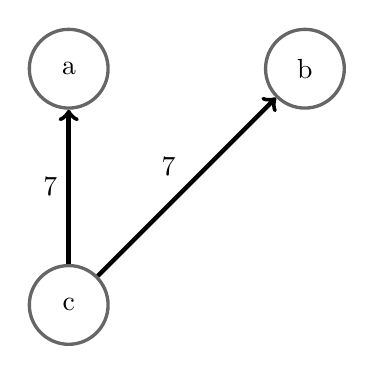
\begin{tikzpicture}[node distance=3cm]
\node [roundnode] (a) {a};
\node [roundnode] (b) [right of=a] {b};
\node [roundnode] (c) [below of=a] {c};
\draw[ultra thick, ->] (c) -- node[auto] {7} (a);
\draw[ultra thick, ->] (c) -- node[auto] {7} (b);
\end{tikzpicture}
\end{center}

In this case, we will observe two sinks in the resulting graph, representing two possible winners.
This corresponds nicely with our intuition of what should happen in this case.

\bigskip

Earlier, we showed how the preference resolution problem can be as simple as finding a sink in a directed graph, an $O(n)$ operation.
Without a guarantee of acyclicity, however, we must turn to alternative methods.
Intuitively, we would like to say that a node which has a lot of incoming edges is preferred, even if that node possesses some number of outgoing edges.

\bigskip

The simplest approach in this vein would be rank items by the value of their incoming edges, with the winner being the item which satisfies $argmax_{v \in V}[in(v)]$.
If the preferences are input as ordered rankings, this method is equivalent to the \textbf{Borda count} election system, a method used in practice by governments today (\cite{reilly:2002}).

\bigskip

A slight variation on this approach would be to take the difference of incoming and outgoing edges, and return the node with the largest difference.
If preferences are input as ordered rankings of all items, this method is equivalent to the method of ranking only the incoming edges.\footnote{For any pair, the sum of incoming and outgoing edges is always equal to the number of votes, therefore $argmax_{v \in V} [in(v) - out(v)] = argmax_{v \in V}[in(v)]$)}
If there is a different access policy, this method may return different results.

These algorithms, which both run in $O(m + n)$ (linear) time, utilize local (pairwise) information between nodes, but incorporate no information about global relationships among nodes.
Given highly structured access policies which constrain the resulting preference graph, these methods are satisfactory.
Given less constrained access policies (in which pairwise preferences are observed at random), these methods will become less reliable, and global methods which incorporate all observed preferences will become necessary.
As we will see, however, algorithms which incorporate global information will take much more than linear time to run.

\subsection{PrefRank}

Google's first PageRank algorithm, designed by founders Sergey Brin and Larry Page, was designed to solve a problem very similar to that of preference resolution: given a directed graph of websites, can one determine which sites are most relevant for a given query?
Brin and Page's solution was to model the web as a random directed graph, and to imagine a \say{random surfer} who would randomly click on links (represented as directed edges from one site to the next).
As this surfer traversed the web, she would be more likely to arrive at pages which had more inbound links; these pages were \textit{preferred}.

Links from preferred pages are worth more than links from peripheral pages, as the popularity of the preferred page meant it was more likely that a surfer would be travel elsewhere via that page.
The PageRank algorithm is nearly identical to the eigenvector-finding techniques discussed above.
The key difference is that PageRank does not include self-edges equal to the indegree of the node, except in the case where the outdegree of a node is $0$ (in order to keep the adjacency matrix full-rank).

\bigskip

The principle difference between the web graph of Brin and Page and the preference graphs we consider here is the variable value associated with the edges.
On the web, a link is a link; there is no notion of a link being worth \say{more} or \say{less}, apart from the page the link originated from.
In our case, edges have weight independent of the popularity of their corresponding nodes.
We can naturally interpret this weight as the strength of the relative preference, and so should seek to allocate preference mass according to the strength of these preferences.

This introduces a complication, however, since the lack of self-edge makes it impossible to consider the popularity of a node when distributing mass away from itself.
By restoring self-edges to the model, we avoid this problem.

\bigskip

We present \textbf{PrefRank}, a extension of PageRank for preference graphs.
PrefRank simply finds the principal eigenvector $v_1$ of a transition matrix $M$, with the results interpreted as a distribution of probabilities $v_1 \in \triangle^{V-1}$.

An eigenvector-based algorithm, our implementation of PrefRank finds $v_1$ using the power method. Each iteration of the power method runs in $O(n^2)$ time, and many iterations may be needed before convergence.
As such, this method is significantly slower than the linear-time methods given above.

\subsubsection{Empirical Results}

We evaluate PrefRank on simulated data as follows.

For $V$ items and preference strength $B$:

\begin{itemize}
	\item for $n \in \{1, ..., N\}$:
	\begin{itemize}
		\item Draw $p_n, q_n$ randomly from $V$.
		\item Draw $\mathbbm{1}[p_n < q_n] \sim Bernoulli(B)$
	\end{itemize}
\end{itemize}

We assess quality of ordering with Spearman's footrule (as discussed in \cite{jordan}), a sum of the per-item position displacements between true ranking and recovered ranking (Figure \ref{fig:pr_0}).

\begin{figure}[!htb]
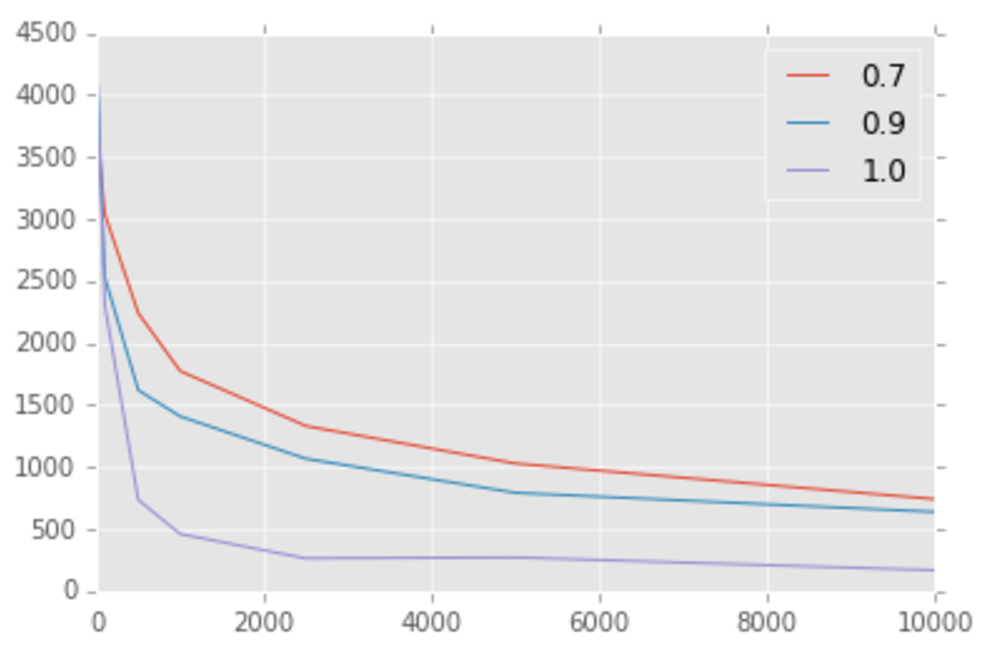
\includegraphics[width=	7cm]{images/pr_100}
\hfill
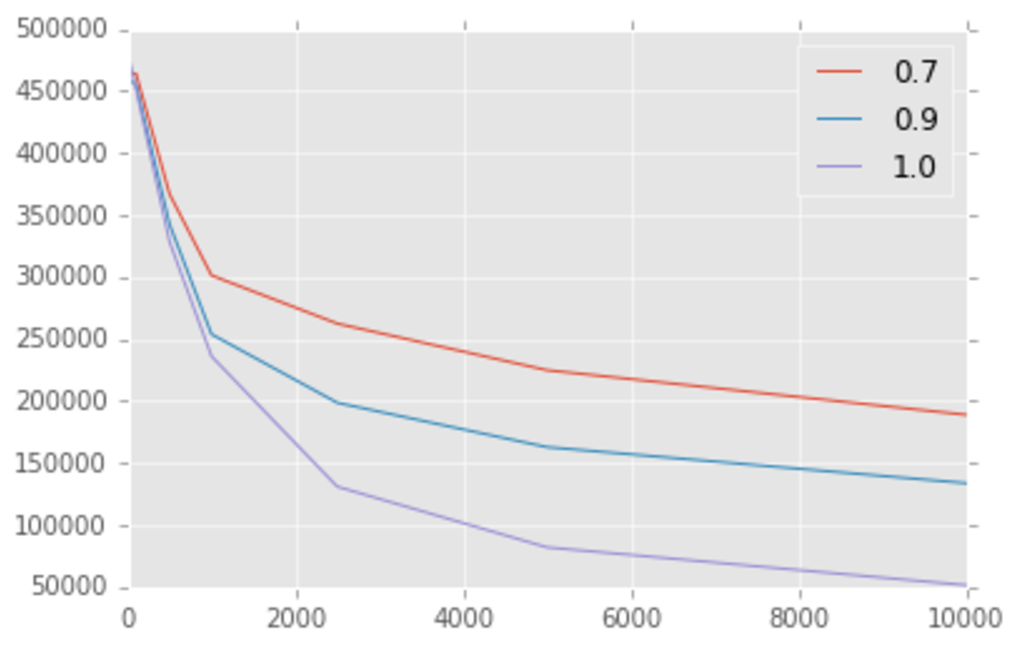
\includegraphics[width=7.2cm]{images/pr_1000}
\caption{Spearman footrule as a function of number of random observations $N$ and a transitive ordering, varying preference strengths B.}
\label{fig:pr_0} 
\end{figure}

\begin{figure}[!htb]
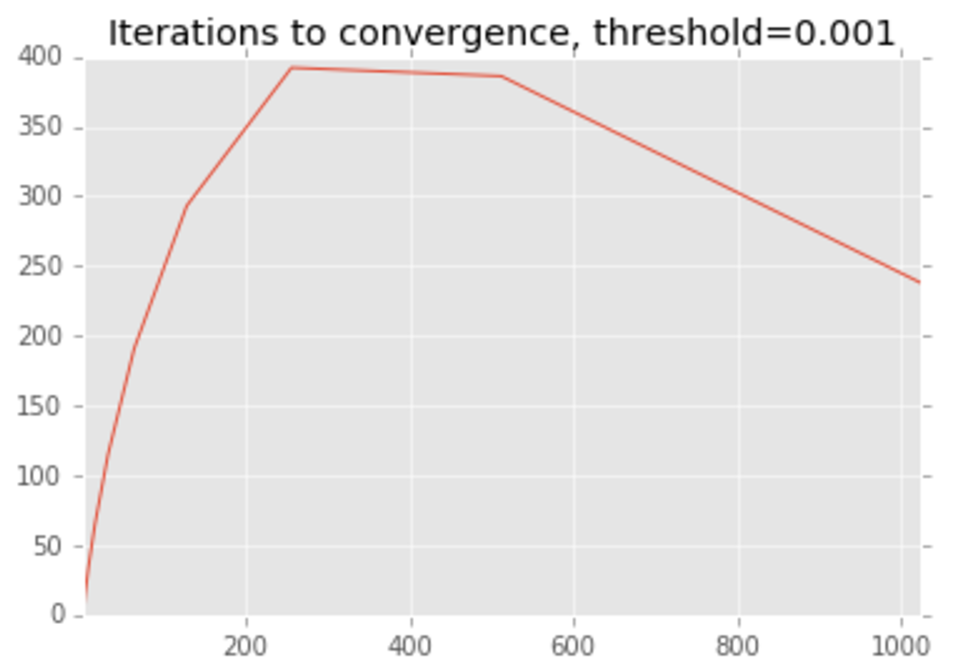
\includegraphics[width=	7cm]{images/pr_iter_001}
\hfill
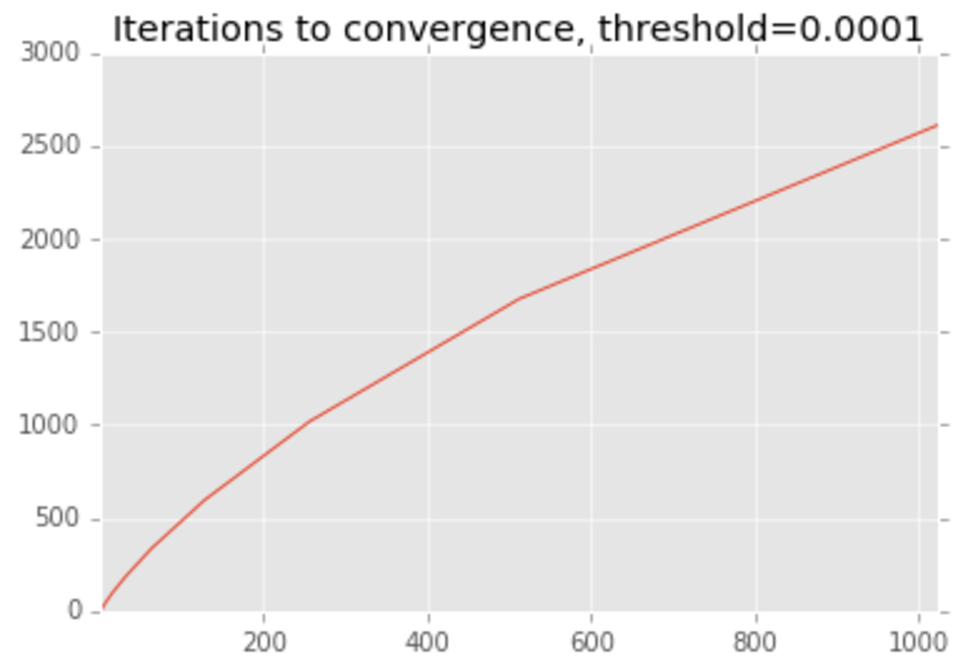
\includegraphics[width=7cm]{images/pr_iter_0001}
\caption{Number of iterations to convergence (given a full set of non-random observations and a transitive ordering) as a function of number of items $|V|$. Initial vector is uniform. The left-hand graph suggests that a larger $n$ requires a lower convergence threshold, as the values will necessarily be smaller.}
\label{fig:pr_1} 
\end{figure}

We conclude that PrefRank is able to recover a large amount of preference structure.
The quality of the structure recovered increases as the number of pairwise observations increases.
Further, the stronger the underlying preference ($B$), the less data was needed to improve accuracy.
These results are unsurprising but bode well.
More work remains to determine under what circumstances and for what specific types of preference does PrefRank perform better.

\subsection{Prototype}

The complexity of the algorithms discussed above are all, in some form, $O(f(n))$.
Finding some way of reducing $n$ would allow all of these techniques to be applied more quickly.

\bigskip

One way to reduce $n$ would be to identify elements of $V$ which are closely related, and to collapse them into more general ``categories'' or ``prototypes,'' which can be treated as though they were single nodes in a graph.
\citet{rosch:1973} provides theoretical justification for this approach, arguing that human cognition utilizes abstract ``prototypes'' in order to reason heuristically about the world.
Identifying these prototypes is conceptually similar to identifying other types of graphical structures, such as communities in social networks.

Community-finding is a major problem in computer science, and much work has been done on this problem.
We present \textbf{Prototype}, an extension of the Mixed-Membership Stochastic Blockmodel (MMSB) of \cite{airoldi:2008} designed to identify such prototypes among a large set of items.

This is a ``Bayesian model'' in that we first assert a model for our data, in which latent factors (hidden variables) interact and ultimately bring about the data we observe.
Inference in this model amounts to learning the optimal (``posterior'') values of these hidden variables, based on the data.

\subsubsection{Model Specification}

In this model, we assume each item is perceived as a mixture of one or more abstract ``prototypes''.
We then assume there is a fixed ``interaction matrix'' $B$, governing preferences between prototypes, where $B_{gh}$ indicates that probability that an item of prototype $h$ is preferred over an item of prototype $g$.

\bigskip

The generative process is as follows:
\begin{itemize}
	\item For items $p \in V$:
	\begin{itemize}
		\item Draw a $K$-dimensional membership vector $\pi_p \sim Dirichlet(\alpha)$.
	\end{itemize}
	\item For each observation $x_n = (p_n, q_n, y_n) \in X$:
	\begin{itemize}
		\item Draw item type $z_{p_n \rightarrow q_n} \sim Multinomial(\pi_{p_n})$
		\item Draw item type $z_{q_n \rightarrow p_n} \sim Multinomial(\pi_{q_n})$
		\item Draw $y_n \sim Bernoulli(z_{p_n \rightarrow q_n}^TBz_{q_n \rightarrow p_n})$
	\end{itemize}
\end{itemize}


Prototype extends the work of \citet{airoldi:2008} by imposing symmetric structure on the matrix $B$.
Specifically, we enforce that $B_{gh} = 1-B_{hg} \; \forall g,h$ (note that this implies $B_{gg}= 0.5 \; \forall g$).
Unlike other mixed-membership stochastic blockmodels, which emphasize intra-community connective patterns, our model exclusively considers inter-community connective patterns.

This model does not attempt to learn distinct preferences per entity.
This was intentional, as this model is attempting to capture and represent preference in aggregate.
That said, this work could be extended by learning a different interaction matrix $B$
per user.
We leave this for future work.

\subsubsection{Inference}

Our goal is to learn posterior values for $\pi_p, z_{p_n \rightarrow q_n}, z_{q_n \rightarrow p_n}$, and $B$.
$\pi_p, z_{p_n \rightarrow q_n}$, and $z_{q_n \rightarrow p_n}$ are random variables, and we will learn posterior values via mean-field variational inference (\cite{wainwright}, \cite{blei:2016}).
$B$ is a matrix of parameters, and so we learn posterior values via variational Expectation-Maximization.

\bigskip

We first assume the following posterior ``$q$'' distributions:

\begin{itemize}
	\item $q(\pi_p) \sim Dirichlet(\gamma_p)$
	\item $q(z_{p_n \rightarrow q_n}) \sim Multinomial(\phi_{p_n \rightarrow q_n})$
	\item $q(z_{q_n \rightarrow p_n}) \sim Multinomial(\phi_{q_n \rightarrow p_n})$
\end{itemize}

The essence of variational inference (specifically coordinate-ascent VI) is that we can learn the optimal distribution of each variable \textit{given the other variables}.
We iterate over the variables, updating their distributions in turn, with each iteration bringing the $q$ distributions closer to the true posterior.

The update equations are as follows:

\[
\hat{\gamma_{p,k}} = \alpha + \sum_{n \in N} \mathbbm{1}(p = p_n)\phi_{p_n \rightarrow q_n,k} + \sum_{n \in N} \mathbbm{1}(p = q_n)\phi_{q_n \rightarrow p_n,k}
\]

\[
\hat{\phi_{p_n \rightarrow q_n,g}} \propto exp\bigg\{\mathbb{E}_q\big[log(\pi_{p,g})\big] + \sum_{h}\phi_{q_n \rightarrow p_n,h}\mathbb{E}_q\big[logp(y_n|B_{gh})\big]\bigg\}
\]

\[
\hat{\phi_{q_n \rightarrow p_n,h}} \propto exp\bigg\{\mathbb{E}_q\big[log(\pi_{q,h})\big] + \sum_{g}\phi_{p_n \rightarrow q_n,g}\mathbb{E}_q\big[logp(y_n|B_{gh})\big]\bigg\}
\]

\[
\hat{B_{gh}} = \frac{
\sum_{n \in N} \phi_{p_n \rightarrow q_n, g} \phi_{q_n \rightarrow p_n, h} y_n + \phi_{p_n \rightarrow q_n, h} \phi_{q_n \rightarrow p_n, g}(1-y_n)
}{
\sum_{n \in N} \phi_{p_n \rightarrow q_n, g} \phi_{q_n \rightarrow p_n, h} + \phi_{p_n \rightarrow q_n, h} \phi_{q_n \rightarrow p_n, g}
}
\]

\bigskip

Additional details of these derivations are given in Appendix \ref{sec:mmsb_appendix}.
Every iteration of the CAVI algorithm has complexity $O(NK^2 + VK)$, again much slower than the linear-time methods.

\subsubsection{Empirical Results}

We evaluated Prototype in three ways: on simulated data, on film review data, and on survey data.
Additional information on these data sources can be found in Appendix \ref{sec:datasets}.

\bigskip

\textbf{Simulations}

\bigskip

In order to validate our implementation and the validity of the model, we fit our MMSB to simulated data.
For small-to-medium sized graphs, our implementation recovers (with some variation) the true prototype distributions $\pi$ and interaction matrix $B$, given enough observations. See Figures \ref{fig:pi_v_gamma} and \ref{fig:interactions_med}.

\bigskip

\textbf{MovieLens Data}

\bigskip

Given that the MovieLens dataset we work with is constructed based on the
user ratings, the preferences we observe for a single user must be transitive.
As such, for a single user, we expect to be able to learn five ``prototypes'', 
each corresponding to a different rating, with the
interaction matrix $B$ to encoding a transitive ordering among these ratings.
We find that this occurs: when setting $K=5$, the model 
learns a strict ordering among the prototypes, and is able to correctly predict 
this user preferences with $98\%$ accuracy on the heldout dataset (Figure \ref{fig:interactions_movie}).  

With multiple users, we are no longer guaranteed a single shared transitive
ordering.
We see in Figure \ref{fig:acc_movies} that the heldout accuracy of the
MMSB plateaus at around $76\%$ when trained on the data from 30 users.
Adding more prototypes, beyond $K=4$, does not improve the
performance of the model. This suggests that the model is simply assigning each
movie to the prototype corresponding to its average rating (and further that there are relatively few movies rated a 1); thus, having more
than 4 or 5 prototypes is not useful.

\bigskip

\textbf{Survey Data}

\bigskip

We fit Prototype to a survey of beer preferences, first considering only the answers from the single opinionated user.
We fit the model to 900 training observations, and measured predictive accuracy on the remaining 344.
We varied K, the number of prototypes, from 1 to 15, but found that predictive accuracy was very stable for $K > 1$, hovering around 78\%.
With $K=3$, our model learned a transitive ordering of preferences among prototypes. See Figure \ref{fig:interactions_beer}.

We next considered the answers coming from all other participants.
We fit the model to 150 training observations and measured accuracy on the remaining 74.
We varied K in the same way as before, and observed both more variable and overall weaker predictive accuracy, rarely surpassing 60\%.
We conclude that this model is capable of capturing prototype interaction structure, but it will not perform well given small samples, weakly structured, or very noisy data.


\begin{figure}
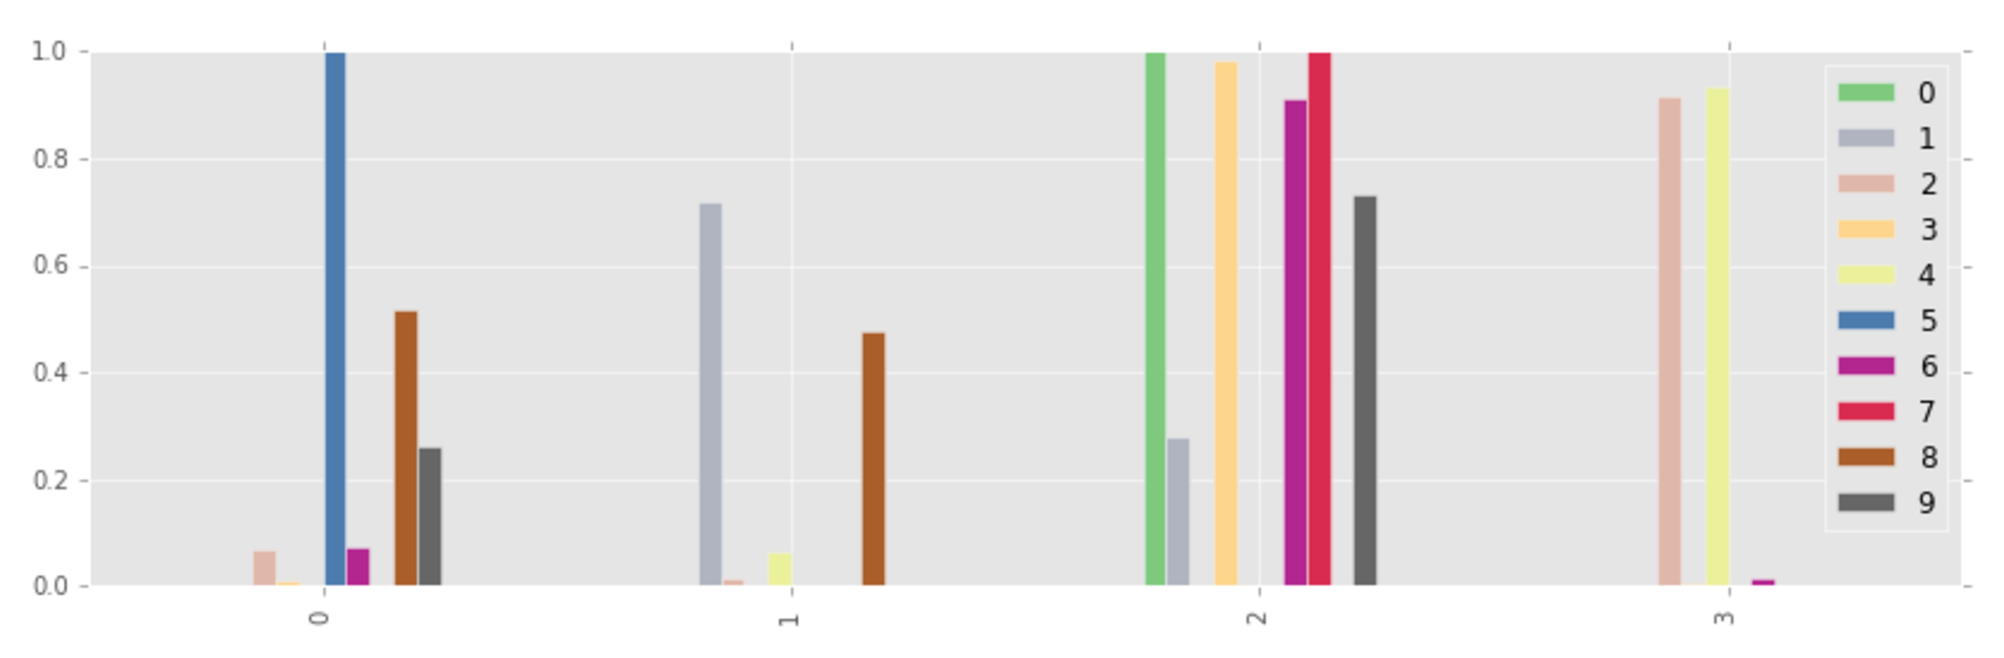
\includegraphics[width=\textwidth]{images/pi}
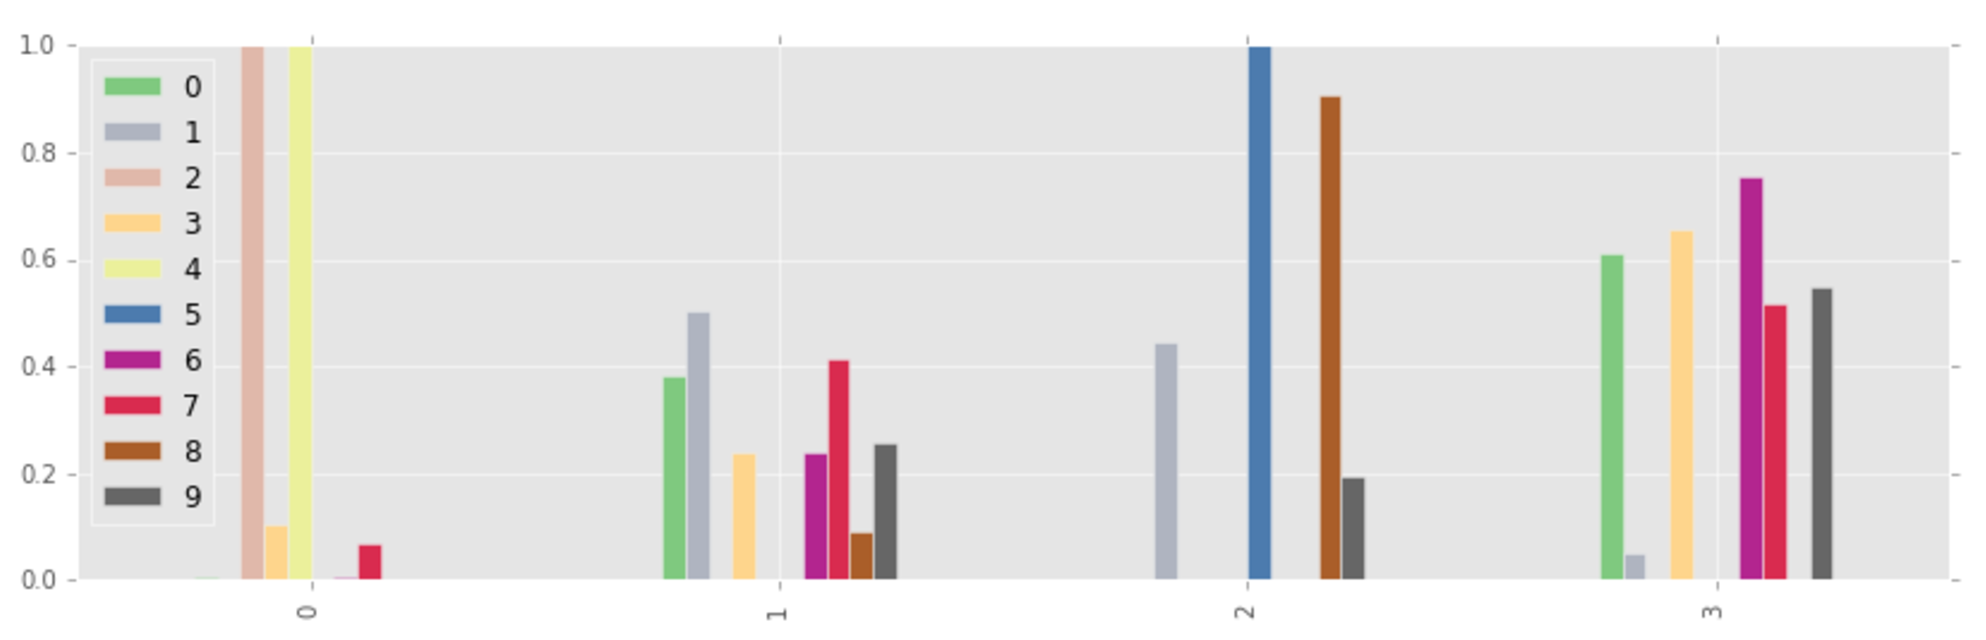
\includegraphics[width=\textwidth]{images/gamma}
\caption{True (top) vs. recovered (bottom) prototype assignments, K=4, V=10, N=10000. We see how the model has correctly grouped the items into their prototypes. Note the label-switching --- this illustrates the multi-modal nature of the joint probability distribution.}
\label{fig:pi_v_gamma} 
\end{figure}


\begin{figure}[!htb]
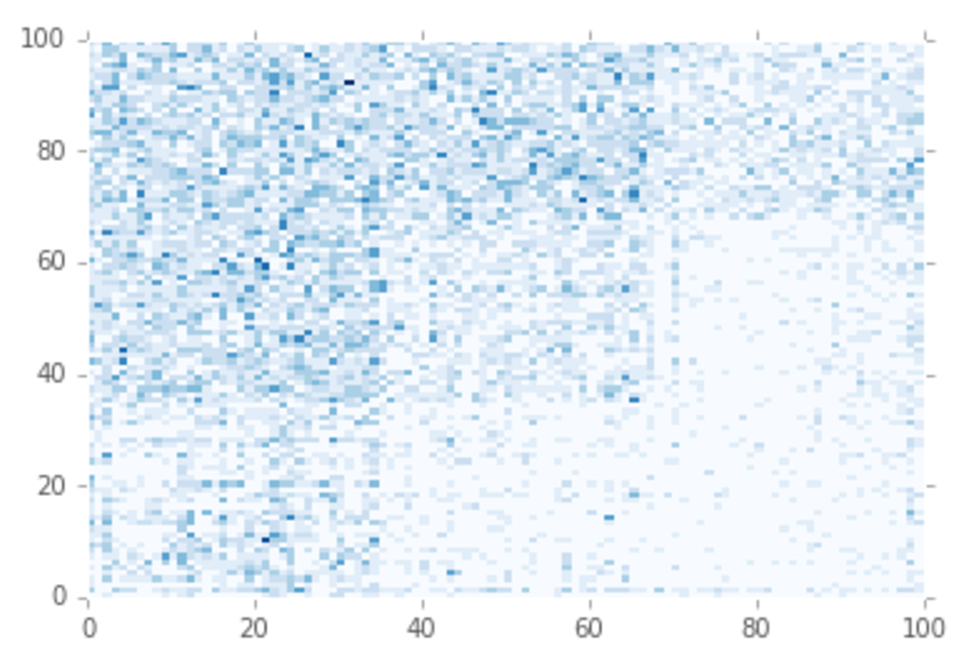
\includegraphics[width=	7cm]{images/10k_5a_95b}
\hfill
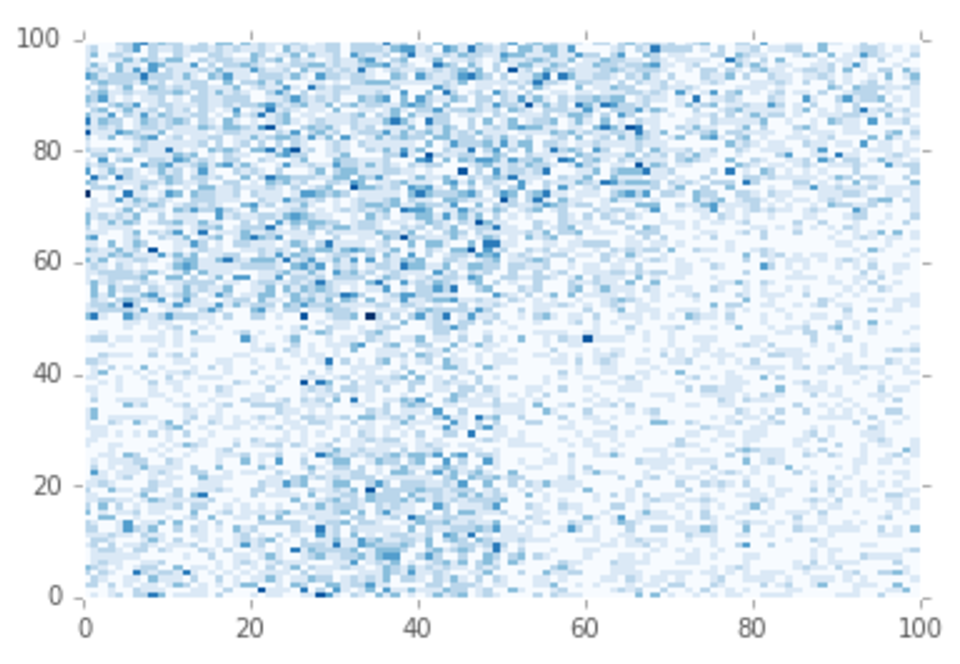
\includegraphics[width=7cm]{images/10k_5a_8b}
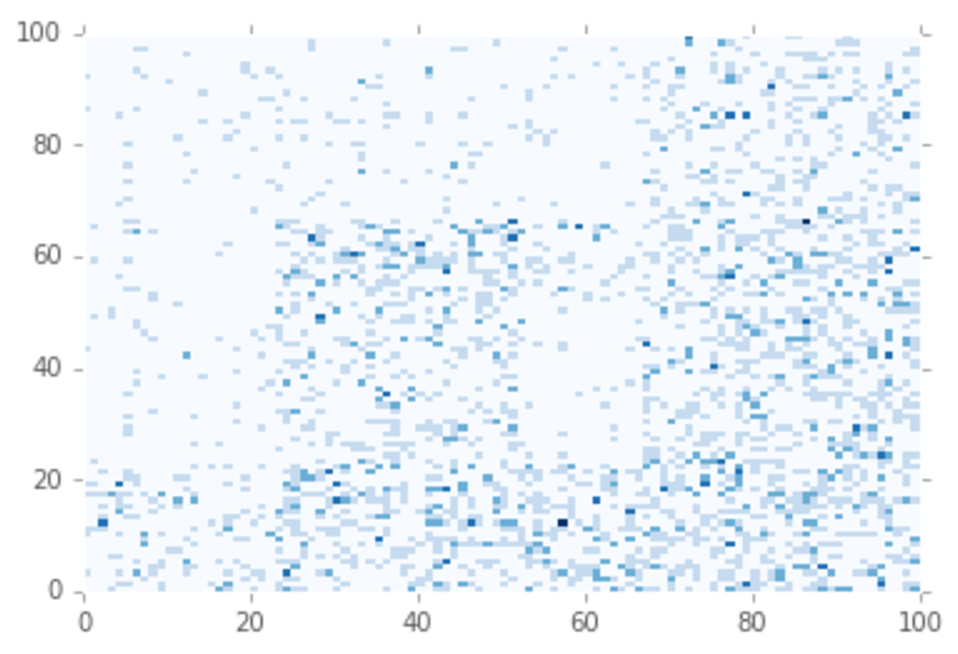
\includegraphics[width=	7cm]{images/2k_5a_95b}
\hfill
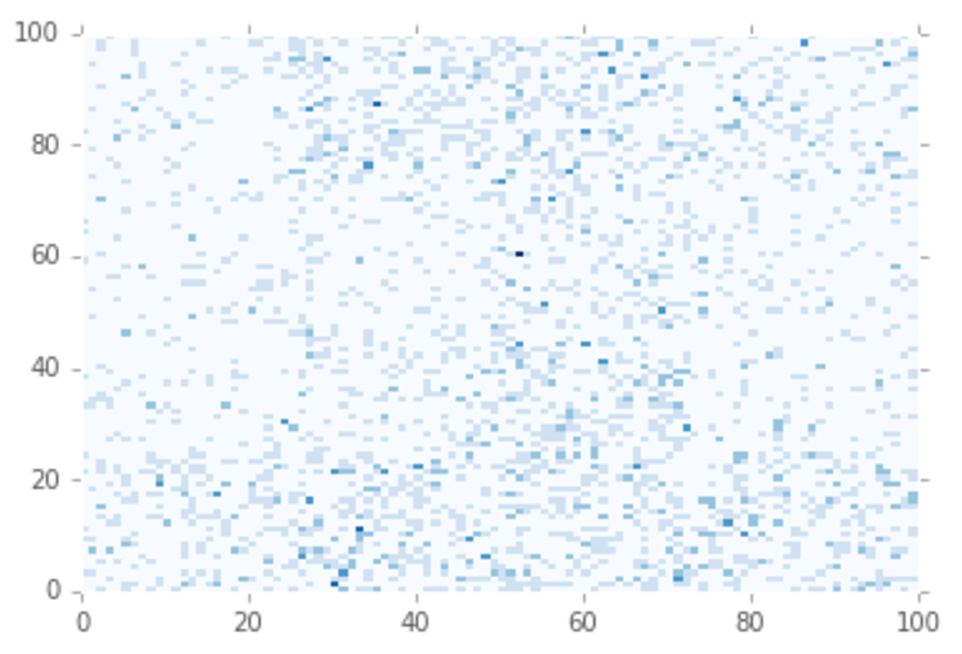
\includegraphics[width=7cm]{images/2k_5a_8b}
\caption{Simulated interaction matrix, items sorted by most likely prototype, K=4, V=100 for all models. Top to bottom: N=1000, 2500. Left to right: B = .95, .8. The visible blocks show that items coming from similar prototypes interact in similar ways to items coming from other prototypes. The diagonal is gray, indicating that intra-prototype comparisons are 50/50 chance.}
\label{fig:interactions_all} 
\end{figure}


\begin{figure}
\centering
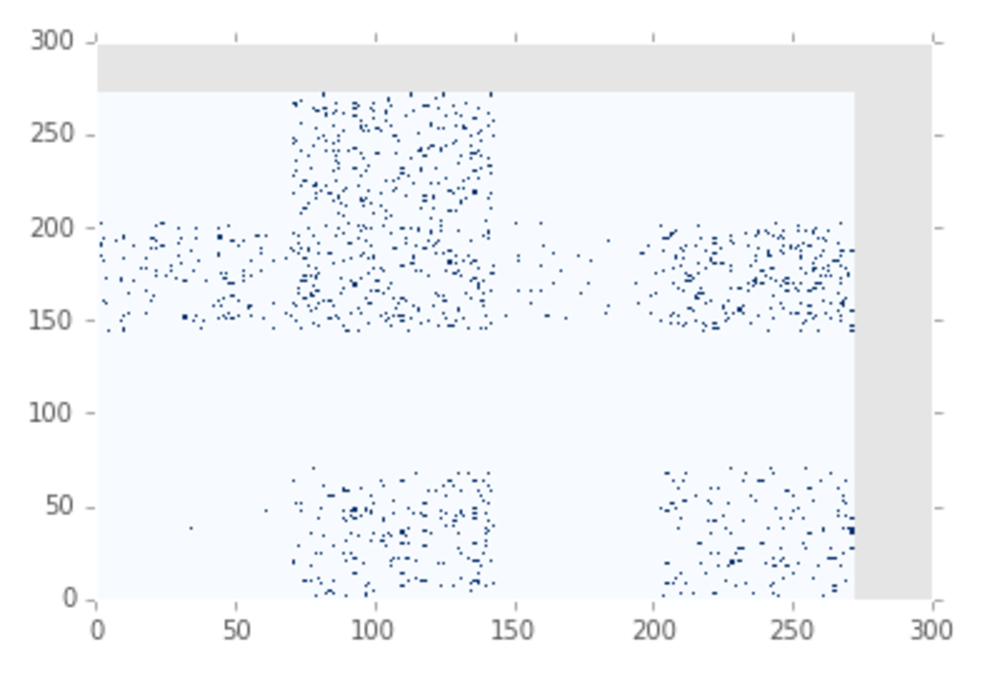
\includegraphics[width=10cm]{images/interactions_movie}
\caption{Movie interaction matrix, one user, items sorted by most likely prototype, K=5, V=272, N=1499}
\label{fig:interactions_movie} 
\end{figure}

\begin{figure}
\centering
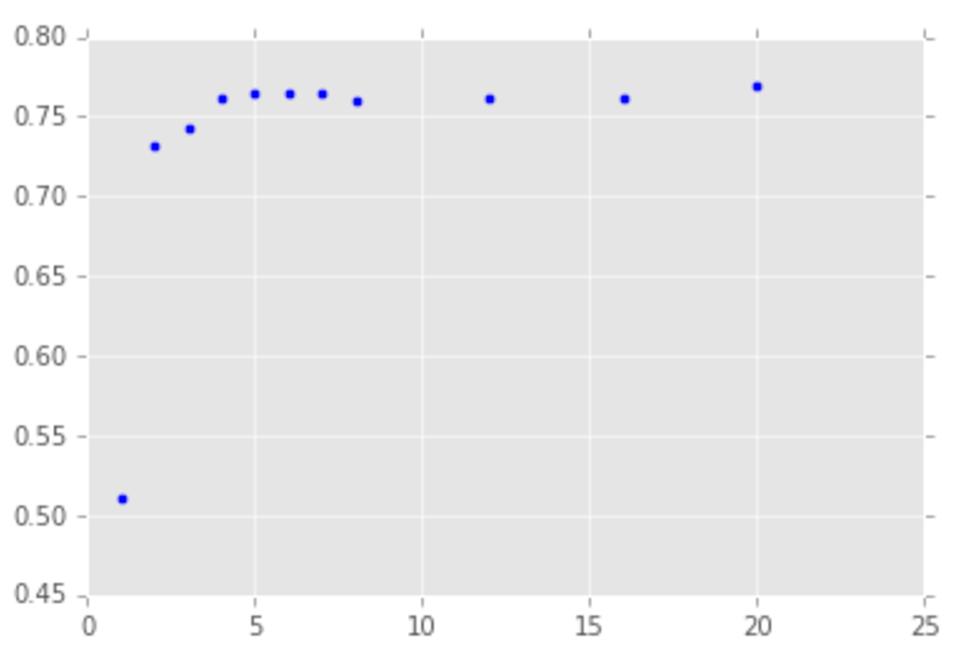
\includegraphics[width=10cm]{images/acc_movies}
\caption{Predictive accuracy against held-out data, 200 films and 20 users, function of number of prototypes $K$. Accuracy plateaus at $K = 4$, suggesting that the model is assigning each movie to a prototype corresponding to an average rating.}
\label{fig:acc_movies} 
\end{figure}


\begin{figure}
\centering
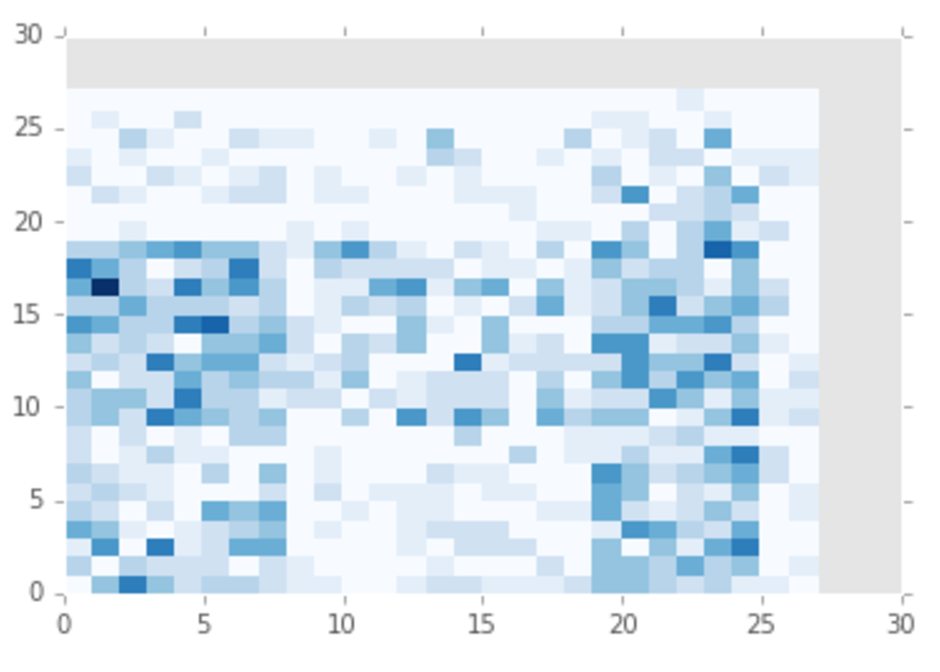
\includegraphics[width=9cm]{images/interactions_beer}
\hfill\raisebox{3cm}{
\begin{tabular}{ | c | c c c | }
\hline
& 0 & 1 & 2 \\ 
\hline
0 & 0.50 & 0.10 & 0.11 \\
1 & 0.90 & 0.50 & 0.89 \\
2 & 0.89 & 0.11 & 0.50 \\
\hline
\end{tabular}
}
\caption{Interaction matrix (left) and B matrix (right) for beer preferences, one user, items sorted by most likely prototype, K=3, V=27, N=1244. We see a transitive ordering of the three prototypes ($1 < 2 < 0$). It is unclear, however, how the items comprising the prototypes should be interpreted.}
\label{fig:interactions_beer} 
\end{figure}

\section{Future Directions}
\subsection{Deployment to a BBVM Environment}

The aim of this work has been to develop methods of representing and analyzing preferences, to facilitate the large-scale coordination of individuals.
In particular, emphasis was placed on understanding the efficiency of analysis.
Efficient analysis would allow for the wider deployment of preference-resolution mechanisms, and their inclusion in a wider range of applications.

\bigskip

In particular, we believe there is opportunity to embed efficient preference-resolution mechanisms into applications deployed to blockchain-based virtual machines, such as Ethereum.
These platforms have the following consequential properties:

\begin{itemize}
	\item The platform is turing-complete, allowing for the performance of computations of arbitrary complexity.
	\item Computations carried out on the platform are redundant and immutable, making results very difficult to fabricate, and therefore highly legitimate.
	\item The platform is distributed, so the system can survive the loss of individual nodes.
\end{itemize}

One could imagine applications which continuously measure and analyze preference, and take autonomous action upon discovering sufficiently clear preference structure.
In general, the fragility of computer systems (susceptibility to hacking, for example), would likely make us reticent to devolve too much decision-making autonomy to these systems.
The resiliency and legitimacy of the BBVM platform, however, make these types of applications more feasible.

\bigskip

The large-scaled redundancy of computation on these platforms (all computations must be carried out by all nodes) means that any analysis run on these platforms will needs be of limited complexity.
This is a major constraint, and motivates the search for more efficient representations and analysis.

The promise here is great, however: were sufficiently efficient representations and analysis discovered, it would be possible to deploy applications which autonomously and legitimately coordinate activity  in a highly non-hierarchical way, without appealing to individual (and therefore susceptible to coercion or exploitation) leadership.
The computational power of these platforms is currently limited, but if the history of computing is any indication (in 1977 the Apple II had RAM measured in kilobytes), they will grow in power over time.
As such, methods of analysis too cumbersome to deploy today may find themselves surprisingly valuable in the years to come.

\subsection{Specialized Access Policies}

In our initial specification of preference graphs mechanics, we discussed the notion of an ``access policy'' governing the creation of preferences.
The simplest access policy would allow any entity to create any preference between any pair of items at any time.
This policy is highly open, but provides few safeguards against manipulation of the preference graph.
Innovations in access policies have the potential to limit the extent to which preference graphs can be manipulated.

One idea would be to incorporate a material cost to preference creation, disincentivizing  entities from creating frivolous preferences.
A related idea would be to tie access to some sort of secondary criteria, such as the ownership of shares in a venture.
In online environments, tying access to material conditions will likely be important in avoiding Sybil attacks \citep{danezis:2006}.

\subsection{Item Pruning and Active Learning}

As discussed earlier, given $n$ items there are $n\choose{2}$ possible pairs.
A larger number of items makes it more difficult to observe a sufficient number of preferences to accurately recover global preference structure.
As such, techniques for either 1) reducing the number of items to be considered, or 2) identifying and observing critical pairs, would help make preference resolution easier for a large number of items.

\subsubsection{Item Pruning}

We have already proposed one method for item pruning, the MMSB algorithm.
This algorithm takes in an arbitrary number of observations and learns $K << n$ prototypes which reflect a higher-level preference structure.
Possession of these prototypes and their relationships reduces the size of the problem in the following ways: 

\begin{itemize}
	\item If there are clear prototypes but complex preferences between prototypes, we can rephrase the question only in terms of the prototypes, easing the problem from complexity in $n$ to complexity in $K$ (``zooming out'').
	\item If there are clear preferences between prototypes, such that one prototype is universally preferred, then we can limit consideration only to the items associated with the winning prototype (``zooming in'').
\end{itemize}

This is only one example.
More techniques for item pruning would allow for the more efficient analysis of complex preference structure.

\subsubsection{Active Learning}

As said, $n$ items creates $n(n-1)/2$ possible pairs.
In this work, we have assumed that preferences will be observed at random, but in practice it is unlikely that all pairs will be of equal importance in discovering preference structure.
For example, if two items seems to be in general preferred over all other items, then we should prioritize learning the relative preference between those two items.
This prioritization is known as ``active learning'' and there exists a large literature on the topic (\cite{shahriari:2016}).

\subsection{Optimal Committee Discovery}

Throughout this work, we have implicitly assumed that larger numbers of entities leads to better, more legitimate decisions.
While this assumption is defensible when considering questions of an abstract or ethical nature (``what is our greatest value'', or ``how should we balance the budget''), this assumption is less defensible when considering technical questions (``how can we improve our energy infrastructure'', or ``which subcontractors should we hire to for this construction project'').
For questions requiring technical expertise, large numbers of non-specialized entities would have noisy and high-entropy (uninformative) preference structure.
It would seem that instead of including the largest number of entities, we should instead seek to assemble a subset of entities (a ``committee'') with the following two properties:

\begin{enumerate}
	\item All entities possess sufficient expertise to be able to make meaningful distinctions between items (nonrandom preference structure).
	\item The variation in preference among these entities adequately covers the variation in preference found in the larger community.
\end{enumerate} 

We would expect preferences drawn from a committee with these properties would be more structured than preferences drawn from the larger community, and therefore easier to analyze and yielding more legitimate conclusions.

\bigskip

The question becomes that of discovering these committees.
One approach would be to pose a question to  all entities, and then consider only the subset of those entities whose preferences meet some criteria for minimal structure (such as having a low tournament entropy or high maximum indegree).
Another approach would be to pose a general question to all entities, and then select those entities whose preferences for the general question meet some criteria, and then put to them the new, more specific question.

\subsection{Question Quality Assessment}

The notion of ``structure'' of preference makes it possible to empirically measure the ``quality'' of a question, with high-quality questions giving rise to highly structured preferences.
In an extreme case, a question consisting of nonsense letters would be expected to lead to completely unstructured answers: entities either abstaining or indicating preferences at random.
Such a question would be low-quality in that it does not give rise to structured preferences.
Following this reasoning, higher-quality questions are those which give rise to more well-structured preferences (however ``structure'' is defined in the context of the particular problem).

If we had two candidate questions $Q_1, Q_2$, and the same set of candidate answers, we could identify objectively the ``better'' question by seeing which question gave rise to more structured preferences.
It is interesting and encouraging to observe how the mechanics of preference graphs given in this work allow us to learn not only the relations between items, but the relations between questions.

\subsection{Conclusions}

The German-American political theorist Hannah Arendt has written about the need for a ``public sphere'', in which there exist methods and structures to allow the achievement of collective freedom via the construction of a common world (\cite{dentreves:2016}).
In Arendt's view, the public sphere is artificial in that does not require grounding in notions of ``natural rights'', but is rather constructed and maintained somewhat arbitrarily by human beings.
Further, Arendt felt that political representation (via elected officials) limited the power of individuals and emphasized the distinction between the rulers and the ruled.
In the spirit of Arendt, we have attempted to lay groundwork for new mechanisms of direct political participation.

\bigskip

This work has explored the question of large-scale nonviolent coordination, taking as its starting point new powerful communication and computational technologies.
We found ourselves closely tracking the work of the social choice theorists, and incorporated ideas from machine learning to attempt to understand and solve those same problems.
We presented a general representation of preference, achieving the goal of formalizing subjectivity.
We then presented a number of algorithms, old and new, for analyzing these types of representations.

\bigskip

One might question the prudence of this line of research.
We appeal to our earlier assertion regarding computing technologies, as well as Arendt's notion of the constructed nature of the public sphere, to conclude that it is fully within our power to discover new ways of living and working together.
In a world stinging from the bitterness of inequality and rapidly losing faith in existing institutions of governance, this line of thinking has never been needed more.

\subsection{Acknowledgements}

We would like to thank Eleni Drinea for her thoughtful advising and valuable feedback on the presentation of a number of technical concepts, Avner May for his assistance in developing the MMSB algorithm, and Steve Bronder for his peer support.
We would also like to thank Steven Kronovet and Stephanie Lehman for graciously opening their 89th street apartment to the author, saving him a number of late-night and early-morning commutes from Bushwick. 


\printbibliography

\end{document}